%\documentclass[prb,twocolumn,showpacs,aps,floats,floatfix,superscriptaddress]{revtex4}
%\documentclass[prb,showpacs,aps,floats,floatfix,superscriptaddress]{revtex4}
%\documentclass{article}
%\documentclass[12pt]{scrreprt}
%\documentclass[onecolumn,letterpaper,amsmath,amssymb,floatfix,aps,superscriptaddress]{revtex4}
\documentclass[a4paper]{article}
\usepackage{epsfig,amsmath,amssymb,array,dcolumn,subfigure,rotating,graphicx}
%\usepackage{graphicx}% Include figure files
%\usepackage{datetime}
\title{\bf Python results: Hamaker coefficients for perpendicular [6,5]
(semi-conductor) cylinders in water using retarded formulation.}
\author{JC Hopkins}
\begin{document}
\maketitle
\begin{abstract}
Comparison of contributions of Matsubara sums to the retarded formulation for\\
Hamaker coeffiecient, ${\cal A}^{(0)}$.  I choose to use [6,5], a
semiiconductor,\\
and [9,3], a semimetal, as examples. All caluclations are for identical pairs
of\\
CNTs in water with a mutual angle of $\pi/2$. \\
\\
Equations correspond to those in version 4 of Rudi's report.
\end{abstract}
\tableofcontents

%%%%%%%%%EPS2 and Aiz%%%%%%%%%%%%%%%%%%%%%%%%%%%%%%%%%%%%%%%%%%%%%%%%
\section{CNT Semi-conductor [6,5]}
\subsection{[6,5] Dielectric response spectrum, dispersion spectrum, and anisotropy measure}
\begin{center}
    From the imaginary part of the dielectric response function of the carbon
nanotubes, \\we compute the London dispersion spectrum by the Kramers-Kronig
transform:
\begin{equation}
\epsilon(i \zeta_n) = 1 + \frac{\pi}{2} \int_0^{\infty} dw
~\frac{\epsilon\prime\prime(\omega)\omega}{\omega^{2} + \zeta^{2}}
\end{equation}
%Where $\zeta_n = 2\pi n k_BT/\hbar$, and $n$ is an integer and the $n=0$ term is counted with a weight $1/2$. 

Relative anisotropy measures in the parallel and perpendicular direction are given by
\begin{equation}
\Delta_{\perp}=\frac{{\epsilon^{c}}_{\perp}-\epsilon_{m}}{{\epsilon^{c}}_{\perp}+\epsilon_{m}}\qquad\Delta_{\parallel}=\frac{{\epsilon^{c}}_{\parallel}-\epsilon_{m}}{\epsilon_{m}}.
\label{anisoind}
\end{equation}

Ratio of anisotropy measure:
\begin{equation}
a_{1,2}(i \omega_n) = \frac{2 \Delta_{\perp}^{(1,2)}(i\omega_n)}{\Delta_{\parallel}^{(1,2)}(i \omega_n)} = 
2 \frac{({{\epsilon^{c}}_{\perp}}^{(1,2)}(i \omega_n) -\epsilon_{m}(i \omega_n)) \epsilon_{m}(i \omega_n)}{({{\epsilon^{c}}_{\perp}}^{(1,2)}(i \omega_n)+\epsilon_{m}(i \omega_n)) ({{\epsilon^{c}}_{\parallel}}^{(1,2)}(i \omega_n) -\epsilon_{m}(i \omega_n))}
\label{eq:adef}
\end{equation}

For interactions between identical CNTs, we set $a_{1}=a_{2}$.  

\begin{figure*}[t!]
\begin{center}
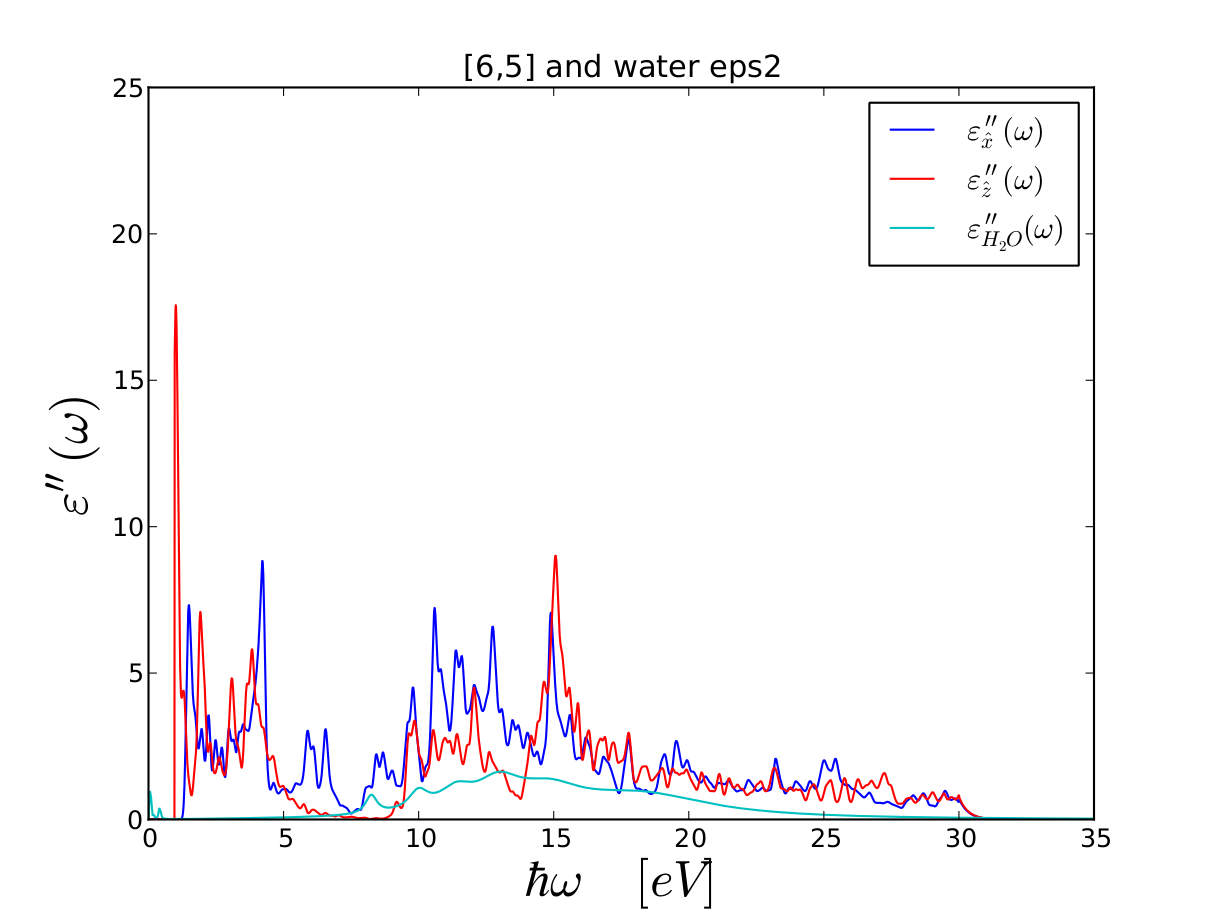
\includegraphics[width=0.8\textwidth]{prop_plots/65w65_eps2.png}
\hskip 43pt
\caption{Imaginary dielectric response spectra for water and the axial and
    radial responses of anisotropic [6,5] CNTs} 
\label{eiz65}
\end{center}
\end{figure*} 

\begin{figure*}[t!]
\begin{center}
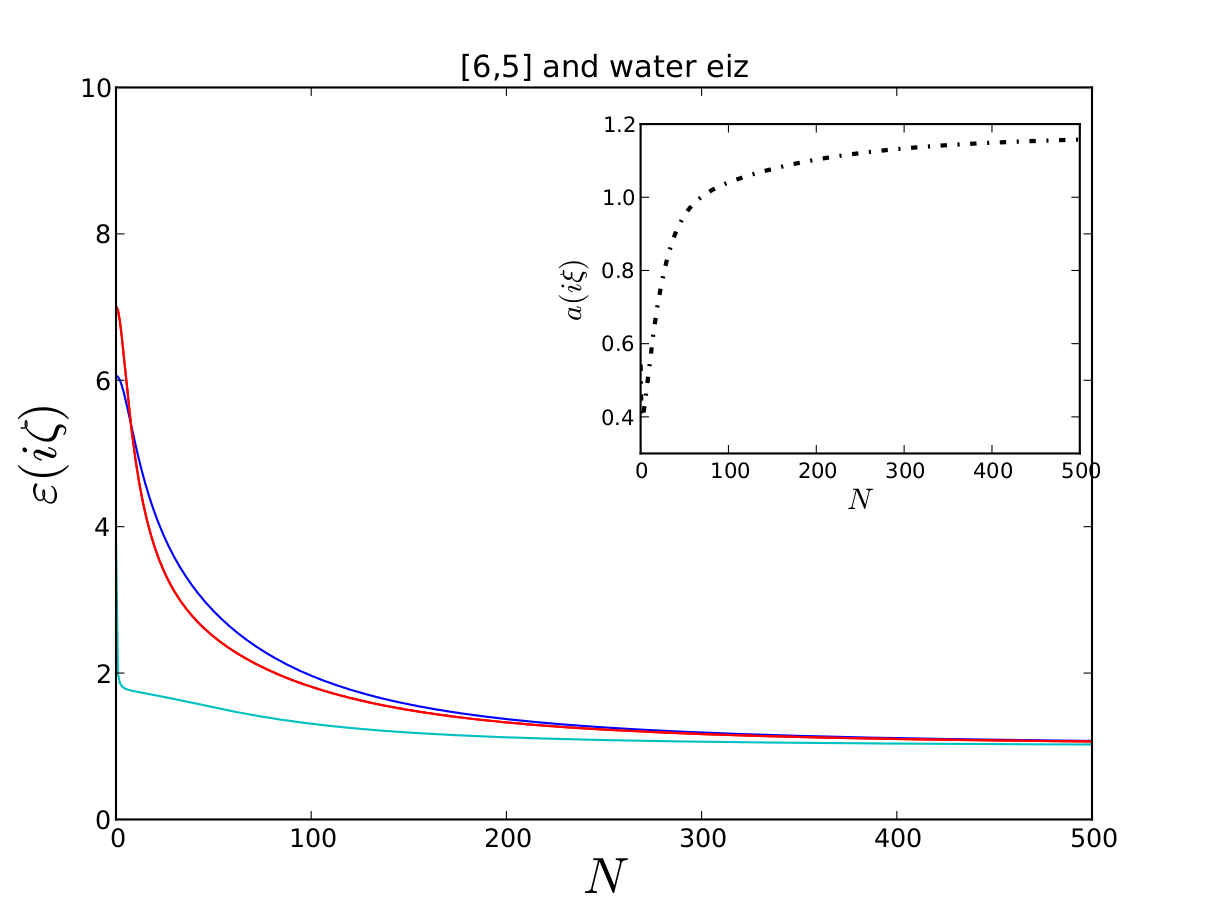
\includegraphics[width=0.8\textwidth]{prop_plots/65w65_eiz.png}
\hskip 43pt
\caption{Dispersion spectrum for anisotropic [6,5] CNT's and
water. The anisotropy measure, $a(i\zeta_n)$, is shown in the inset.} 
\label{eiz65}
\end{center}
\end{figure*} 

\end{center}
%\begin{figure*}[t!]
%\begin{center}
%\begin{minipage}[b]{0.40\textwidth}
%\begin{center}
%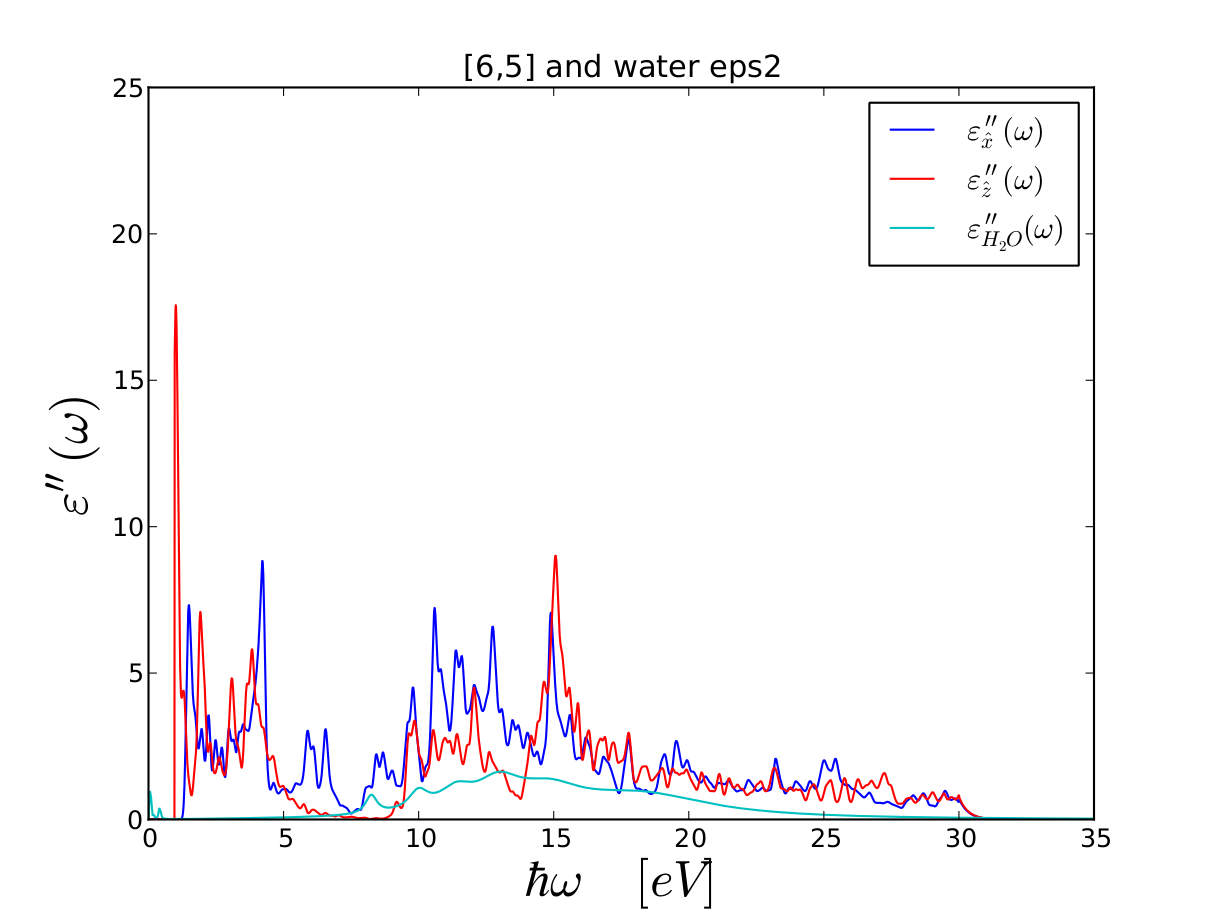
\includegraphics[width=1.4\textwidth]{prop_plots/65w65_eps2.png} (a)
%\end{center}
%\end{minipage}
%\hskip 43pt
%\begin{minipage}[b]{0.40\textwidth}
%\begin{center}
%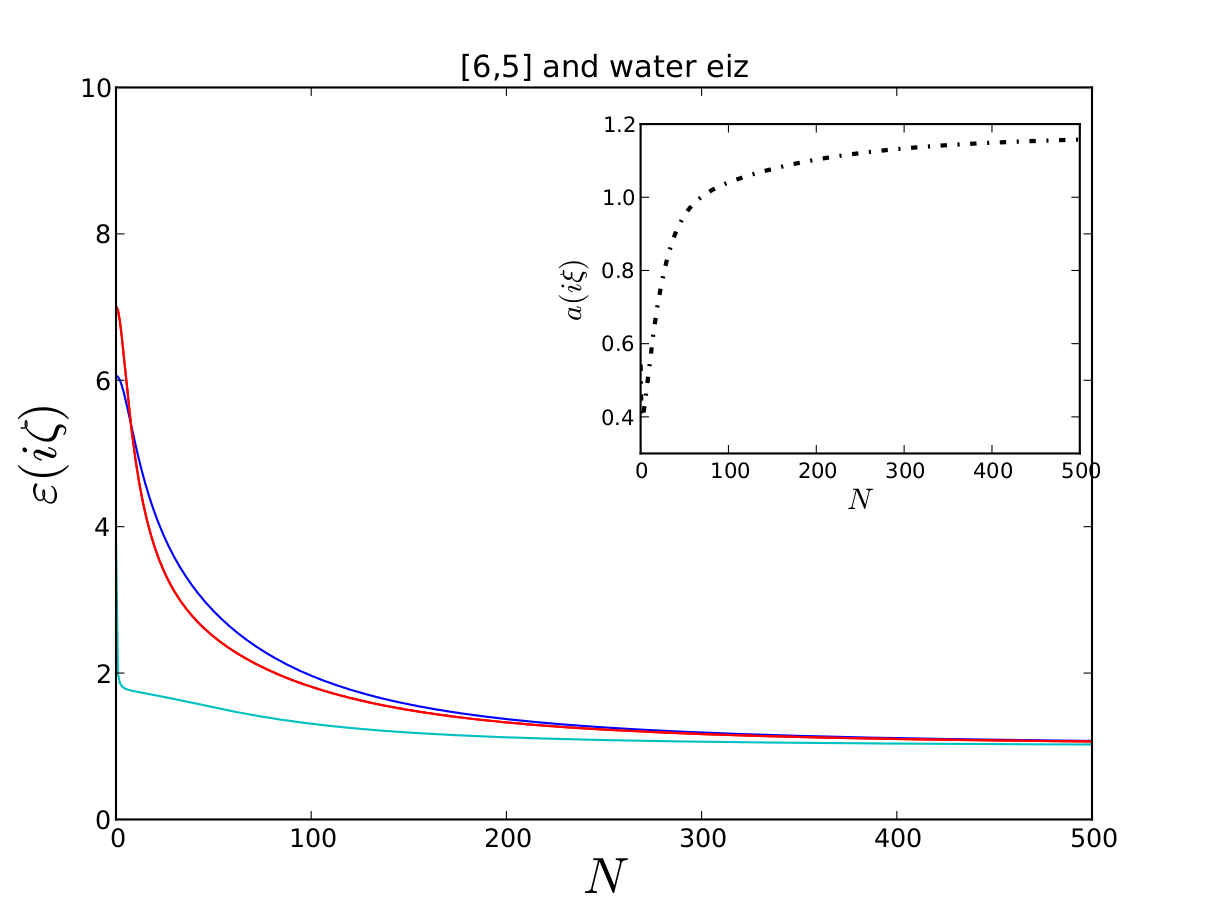
\includegraphics[width=1.4\textwidth]{prop_plots/65w65_eiz.png} (b)
%\end{center}
%\end{minipage}
%\caption{(a) Imaginary dielectric response spectrum, (b) dispersion spectrum and anisotropy measure (inset)}
%\label{eiz65}
%\end{center}
%\end{figure*}

\subsection{[6,5] Dielectric contrast, anisotropy measure, and their derivatives}
\begin{center}
The relative anisotropy compares the dielectric contrasts, $\Delta$, of the\\ 
radial and axial responses of the CNTs in water.\\
\smallskip{}
For interactions between identical CNTs, we set $a_{1}=a_{2}$.\\  

\smallskip{}
The ratio of anisotropy measure is given as
\begin{equation}
a_{1,2}(i \omega_n) = \frac{2 \Delta_{\perp}^{(1,2)}(i\omega_n)}{\Delta_{\parallel}^{(1,2)}(i \omega_n)} = 
2 \frac{({{\epsilon^{c}}_{\perp}}^{(1,2)}(i \omega_n) -\epsilon_{m}(i \omega_n)) \epsilon_{m}(i \omega_n)}{({{\epsilon^{c}}_{\perp}}^{(1,2)}(i \omega_n)+\epsilon_{m}(i \omega_n)) ({{\epsilon^{c}}_{\parallel}}^{(1,2)}(i \omega_n) -\epsilon_{m}(i \omega_n))}
\label{eq:adef}
\end{equation}
where the dielectric contrasts are given by
\begin{equation}
\Delta_{\perp}=\frac{{\epsilon^{c}}_{\perp}-\epsilon_{m}}{{\epsilon^{c}}_{\perp}+\epsilon_{m}}\qquad\Delta_{\parallel}=\frac{{\epsilon^{c}}_{\parallel}-\epsilon_{m}}{\epsilon_{m}}.
\label{anisoind}
\end{equation}
\\
For the sake of completeness, I have plotted the behaviors of $\Delta$ and\\
$a(i\zeta)$ as they appear in the equations for Hamaker Coefficients as well as
their derivatives with respect to n.
\begin{figure*}[t!]
\begin{center}
    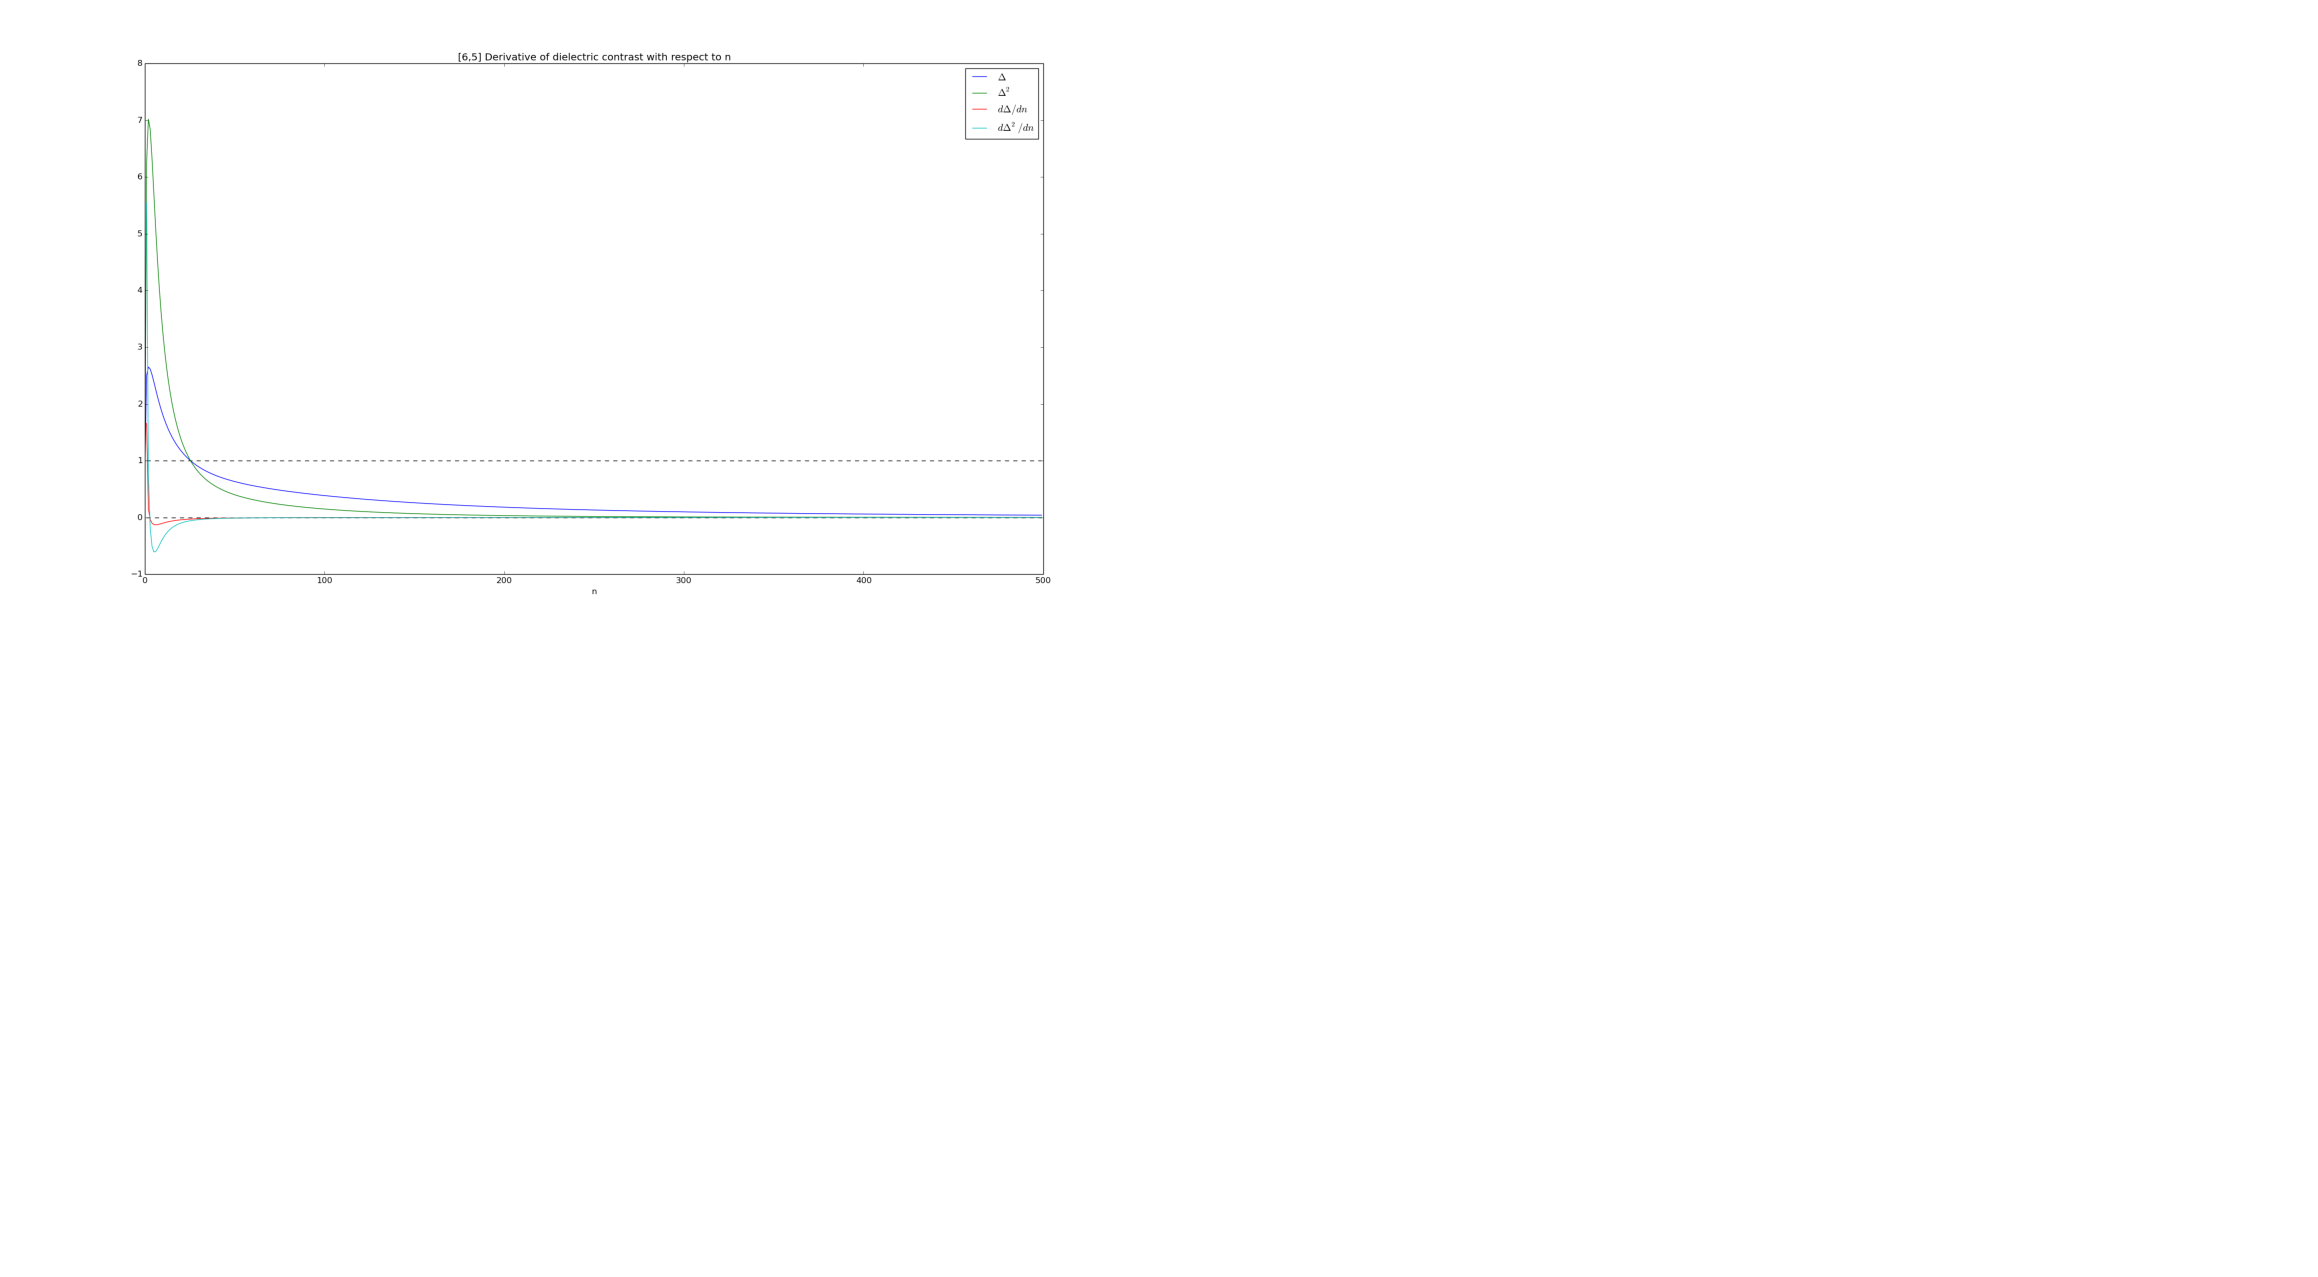
\includegraphics[width=0.8\textwidth,scale= 0.8]{plots/delta_derivs_65.png}
\hskip 43pt
\caption{Dielectric contrast of [6,5] CNTs in water, its square, and their
derivatives with respect to n.} 
\label{eiz65}
\end{center}
\end{figure*} 

\begin{figure*}[t!]
\begin{center}
    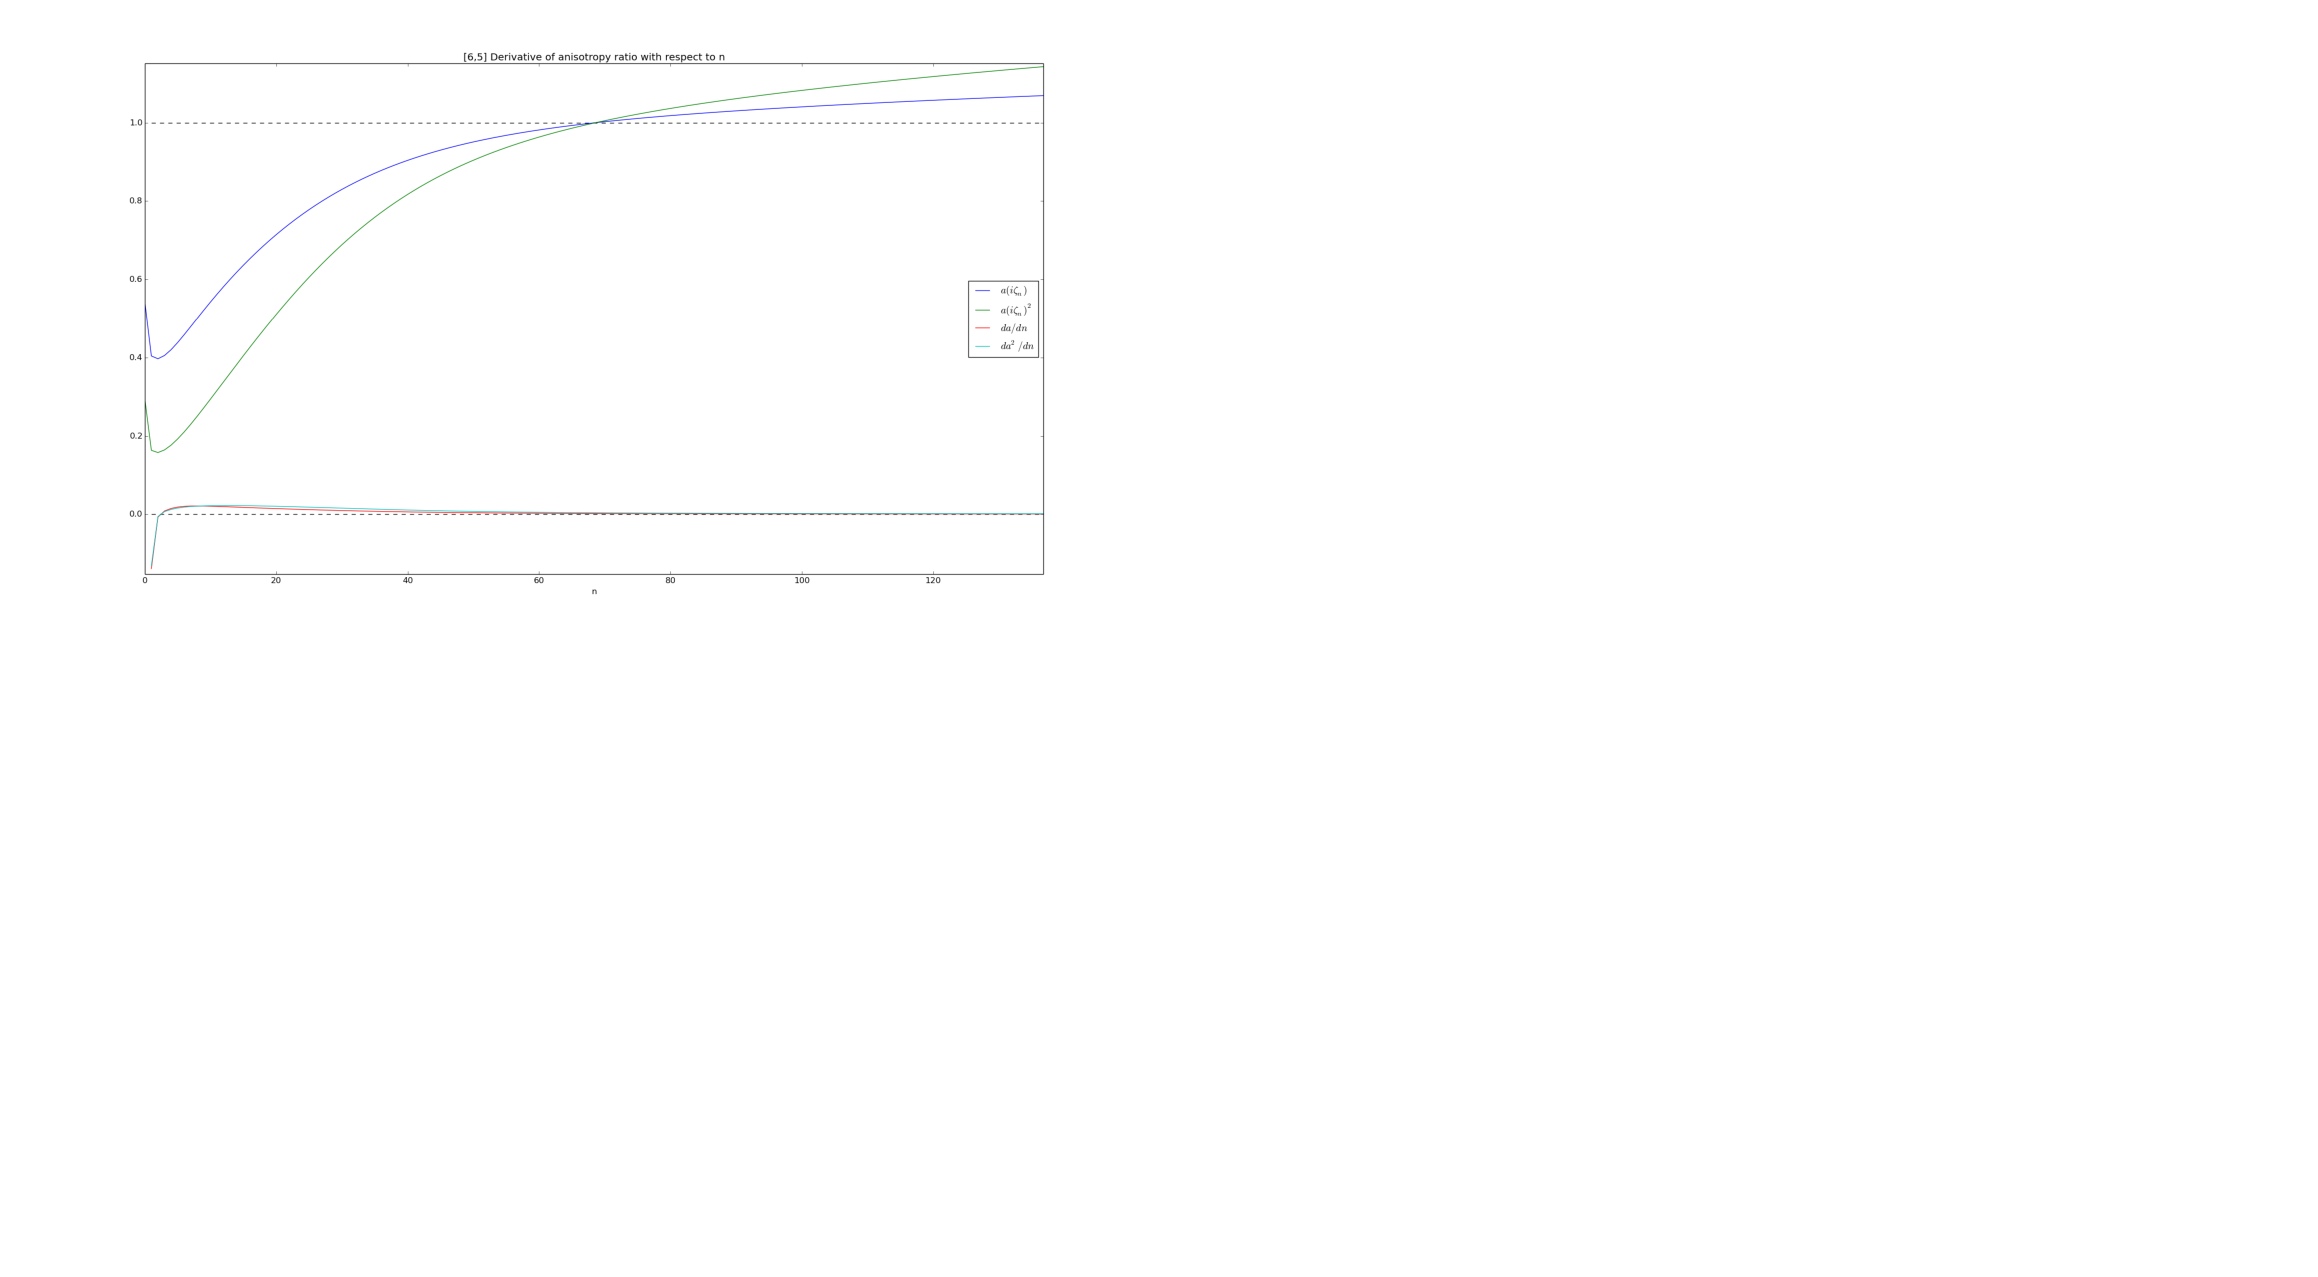
\includegraphics[width=0.8\textwidth,scale= 0.8]{plots/a_derivs_65.png}
\hskip 43pt
\caption{Anisotropy ratio of [6,5] CNTs in water, its square, and their
derivatives with respect to n.} 
\label{eiz65}
\end{center}
\end{figure*} 
\end{center}

%%%%%%%%%%%%%%%%%%%%%%%%%%%%%%%%%[6,5] HAMAKERS %%%%%%%%%%%%%%%%%%%%%%%%%%%%%%%
\subsection{[6,5] Fully retarded Hamaker Coefficients for Matsubara Sum }
\begin{center}
Using equations from v.4 of Rudi's report, we calculate the fully retarded\\ 
Hamaker coefficients for perpendicular, identical [6,5] CNTs in water, as given
by:
\begin{equation}
{\cal A}^{(0)}(\ell) = \frac{k_BT}{32}  {\sum_{n=0}^{\infty}}' \Delta_{1,\parallel} \Delta_{2,\parallel} ~p_n^{4}(\ell) ~\int_0^{\infty} t dt ~\frac{e^{- 2 p_n(\ell) \sqrt{t^{2} + 1}}}{(t^{2} + 1)} \tilde g^{(0)}(t, a_1(i \omega_n), a_2(i \omega_n))
\end{equation}

\begin{multline*}
\tilde g^{(0)}(t, a_1(i \omega_n), a_2(i \omega_n)) = \\ 
2 \left[ (1+3a_1)(1+3a_2) t^{4} + 2 (1+2a_1+2a_2+3a_1a_2) t^{2}  + 2(1+a_1)(1+a_2)\right]
\end{multline*}
and
\begin{equation}
{\cal A}^{(2)}(\ell) = \frac{k_BT}{32}  {\sum_{n=0}^{\infty}}' \Delta_{1,\parallel} \Delta_{2,\parallel} ~p_n^{4}(\ell) ~\int_0^{\infty} t dt ~\frac{e^{- 2 p_n(\ell) \sqrt{t^{2} + 1}}}{(t^{2} + 1)} \tilde g^{(2)}(t, a_1(i \omega_n), a_2(i \omega_n), \theta)
\end{equation}

\begin{equation}
\tilde g^{(2)}(t, a_1(i \omega_n), a_2(i \omega_n), \theta) = (1-a_1)(1-a_2)(t^{2} + 2)^2
\label{befgqw}
\end{equation}
with the n = 0 term given by
\begin{equation}
    {\cal A}_{n=0}^{(0)}(\ell) = \frac{1}{2} \frac{k_BT}{32}
    \Delta_{1,\parallel} \Delta_{2,\parallel} ~\int_0^{\infty} u^3 du\,\,
    e^{-2u}\,\,[2(1 + 3a_1)(1 + 3a_2) ]
\end{equation}
and
\begin{equation}
    {\cal A}_{n=0}^{(2)}(\ell) = \frac{1}{2} \frac{k_BT}{32}
    \Delta_{1,\parallel} \Delta_{2,\parallel} ~\int_0^{\infty} u^3 du\,\,
    e^{-2u}\,\,[(1 - a_1)(1 - a_2) ]
\end{equation}
where $u = Ql$.

\hskip 73pt
The two figures below give the fully retared Hamaker coefficents,\\ 
${\cal A}^{(0)}$ and ${\cal A}^{(2)}$, as a function of separation.\\
\hskip 73pt
Log-log plot of Hamaker coeffcients as a function of separation:
\begin{figure*}[t!]
\begin{center}
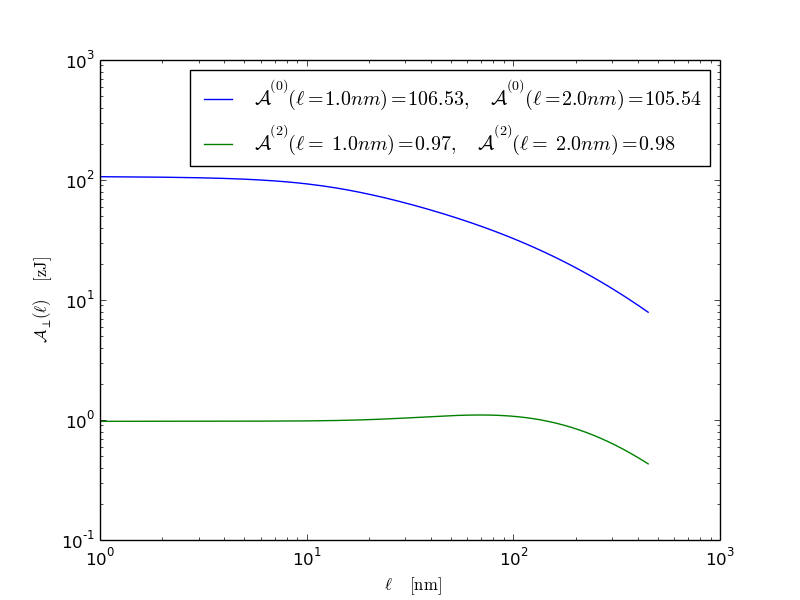
\includegraphics[width=1.2\textwidth]{plots/140322_65w65_HCs_perpendicular_ret.png}
%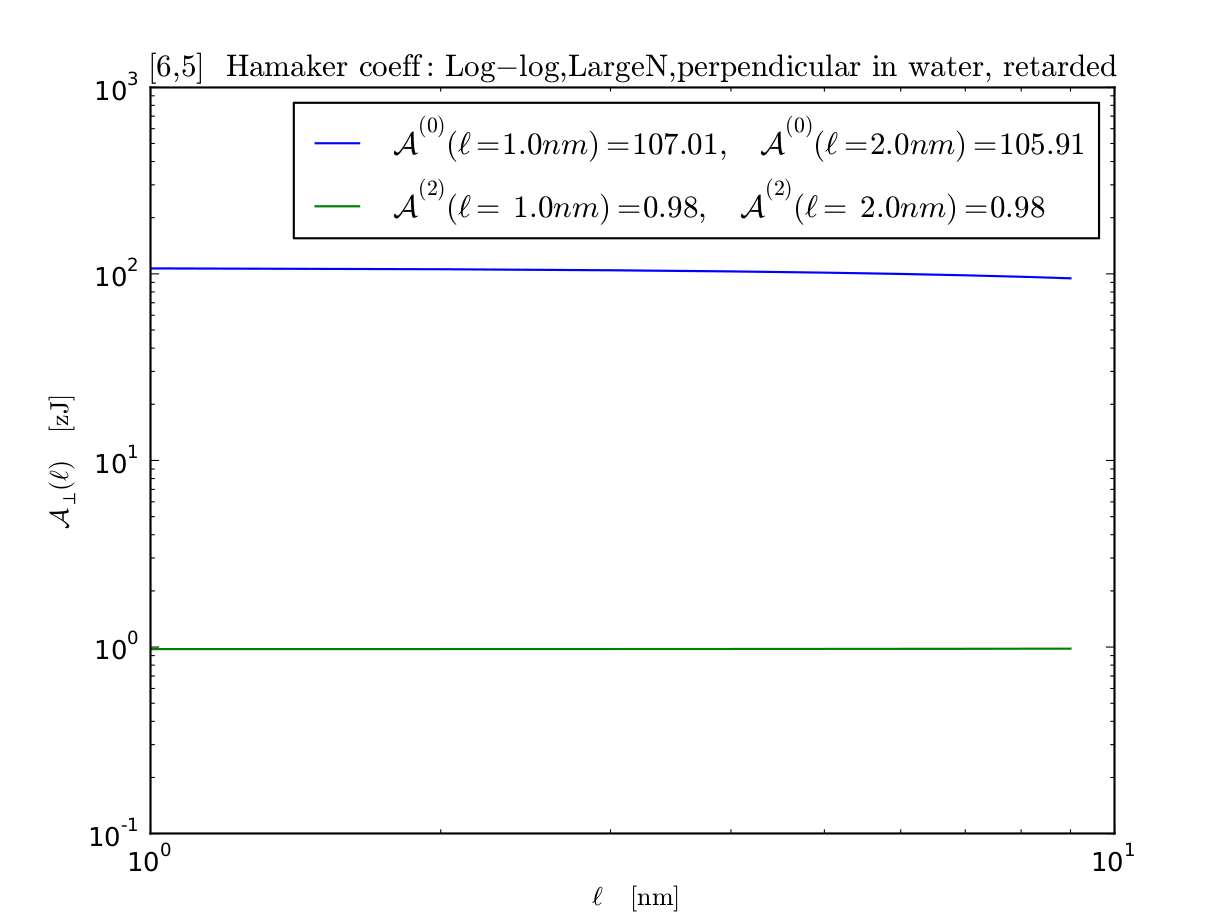
\includegraphics[width=1.2\textwidth]{large_N/140322_65w65_HCs_perpendicular_ret_lrg_n.png}
\hskip 43pt
\caption{Log-log plot of fully retarded Hamaker coeffiecents for perpendicular, identical [6,5] CNT's in water
as a function of separation.} 
\label{eiz65}
\end{center}
\end{figure*} 

\hskip 73pt
%%%%%%%%%%%%%%%%%%%%%%%%%%%%%%%%% SEMILOG A %%%%%%%%%%%%%%%%
Semi-log plot of Hamaker coeffcients as a function of separation:
\begin{figure*}[t!]
\begin{center}
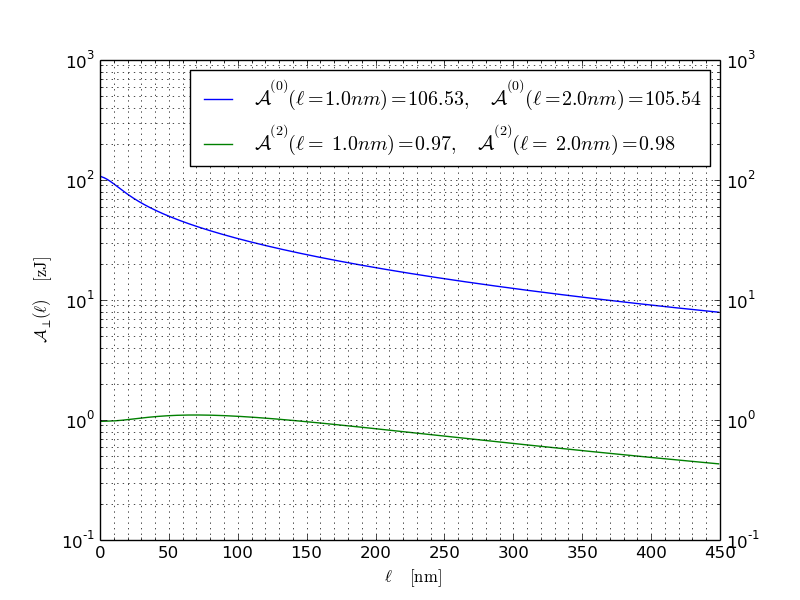
\includegraphics[width=1.2\textwidth]{plots/140322_65w65_HCs_semilog_perpendicular_ret.png}
%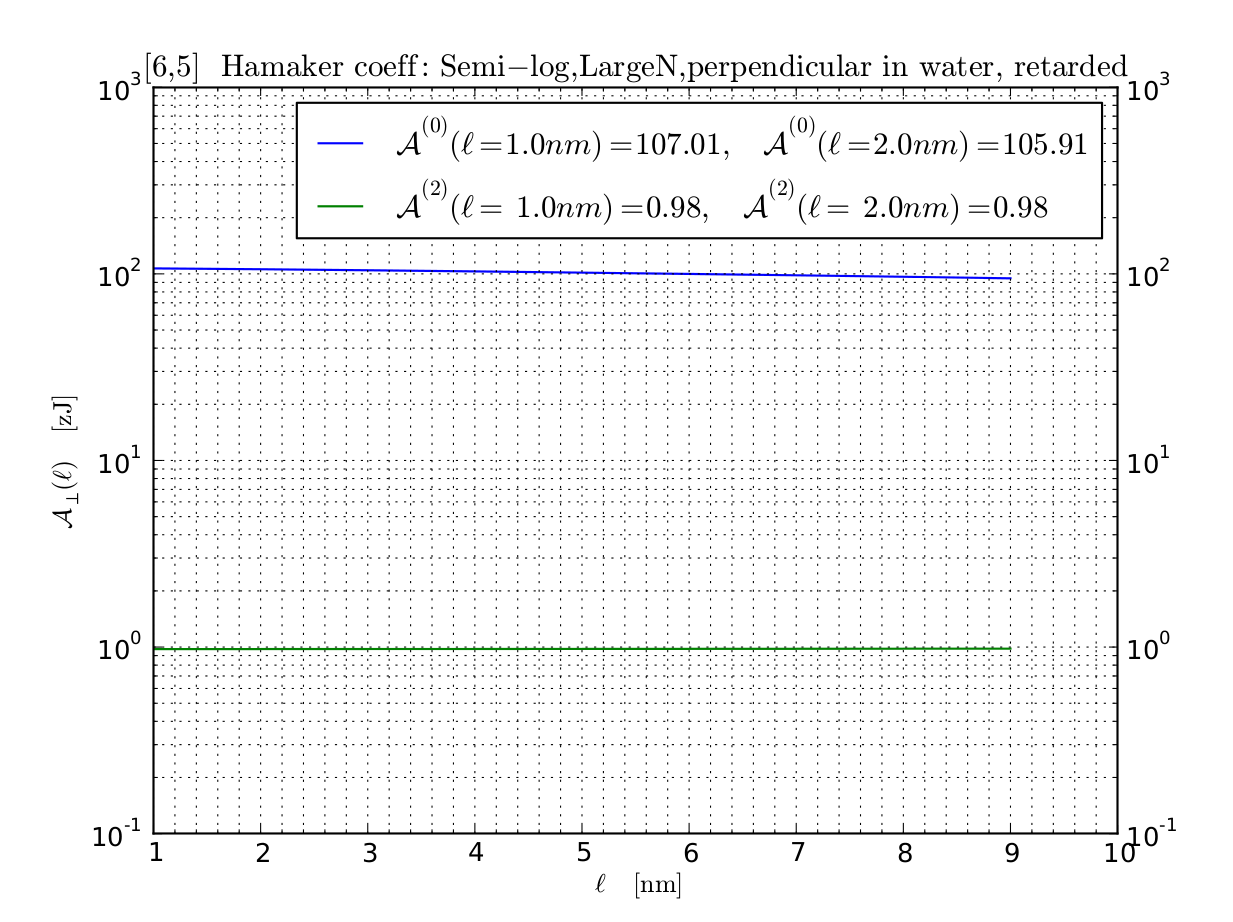
\includegraphics[width=1.2\textwidth]{large_N/140322_65w65_HCs_semilog_perpendicular_ret_lrg_n.png}
\hskip 43pt
\caption{Semi-log plot of fully retarded Hamaker coeffiecents for perpendicular, identical [6,5] CNT's in water
as a function of separation.} 
\label{eiz65}
\end{center}
\end{figure*} 
\end{center}

%%%%%%%%%%%%%%%%%%%%%%%%%%%%%%%%% 65 Terms of A %%%%%%%%%%%%%%%%
\subsection{[6,5] Terms of Matsubara sum and their derivatives with respect to
$\ell$ and $n$}
\begin{center}
We investigate the amount that each term contributes to the Matsubara sum, in\\
the Hamaker coefficents, ${\cal A}^{(0)}$ and ${\cal A}^{(2)}$.
\begin{equation}
{\cal A}^{(0)}(\ell) = \frac{k_BT}{32}  {\sum_{n=0}^{\infty}}' \Delta_{1,\parallel} \Delta_{2,\parallel} ~p_n^{4}(\ell) ~\int_0^{\infty} t dt ~\frac{e^{- 2 p_n(\ell) \sqrt{t^{2} + 1}}}{(t^{2} + 1)} \tilde g^{(0)}(t, a_1(i \omega_n), a_2(i \omega_n))
\end{equation}
and
\begin{equation}
{\cal A}^{(2)}(\ell) = \frac{k_BT}{32}  {\sum_{n=0}^{\infty}}' \Delta_{1,\parallel} \Delta_{2,\parallel} ~p_n^{4}(\ell) ~\int_0^{\infty} t dt ~\frac{e^{- 2 p_n(\ell) \sqrt{t^{2} + 1}}}{(t^{2} + 1)} \tilde g^{(2)}(t, a_1(i \omega_n), a_2(i \omega_n), \theta)
\end{equation}
with the n = 0 term given by
\begin{equation}
    {\cal A}_{n=0}^{(0)}(\ell) = \frac{1}{2} \frac{k_BT}{32}
    \Delta_{1,\parallel} \Delta_{2,\parallel} ~\int_0^{\infty} u^3 du\,\,
    e^{-2u}\,\,[2(1 + 3a_1)(1 + 3a_2) ]
\end{equation}
and
\begin{equation}
    {\cal A}_{n=0}^{(2)}(\ell) = \frac{1}{2} \frac{k_BT}{32}
    \Delta_{1,\parallel} \Delta_{2,\parallel} ~\int_0^{\infty} u^3 du\,\,
    e^{-2u}\,\,[(1 - a_1)(1 - a_2) ]
\end{equation}
where $u = Ql$.

\hskip 73pt
The following plot shows the value of each term of ${\cal A}$ for different values of separations. As separations increase,\\ 
more of the higher frenquency terms of ${\cal A}^{(0)}$ show a weakened contribution to the sum.\\
\smallskip{}

\begin{figure*}[t!]
\begin{center}
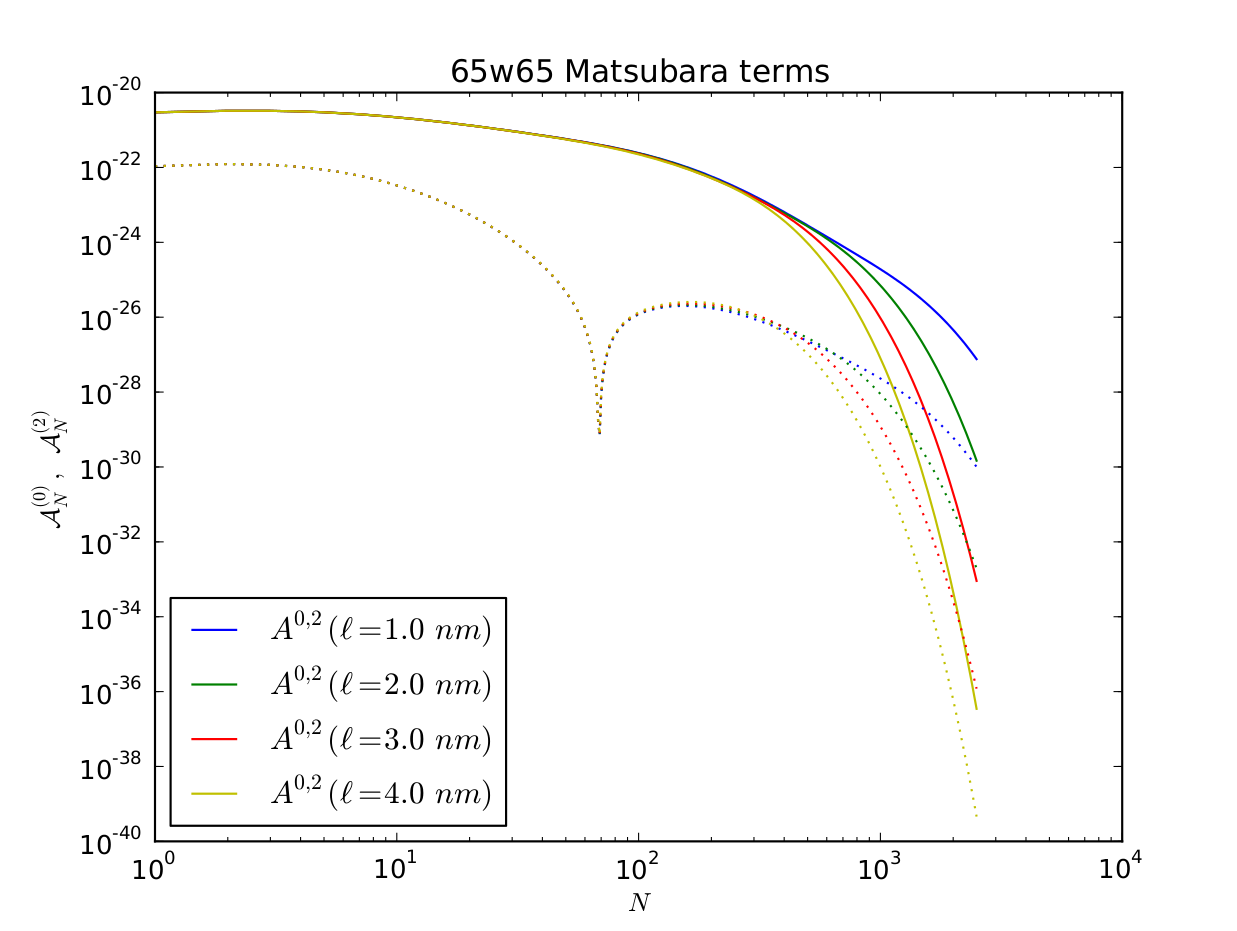
\includegraphics[width=1.2\textwidth,scale= 0.7]{large_N/65_A_vs_lrg_n.png}
\hskip 43pt
\caption{\bf{Terms contributing to Matsubara sum as a function of n.}
    The terms of ${\cal A}^{(2)}$ show a sharp valley at the value of n for which the
dispersion spectra, $\epsilon_{\perp}$ and $\epsilon_{\parallel}$, have
their closest approach to each other.}
\label{eiz65}
\end{center}
\end{figure*} 
\hskip 73pt
%%%%%%%%%%%%%% 65 dA0/dl %%%%%%%%%%%%%%%%%%%%%%%%%%%%%%
\begin{figure*}[t!]
\begin{center}
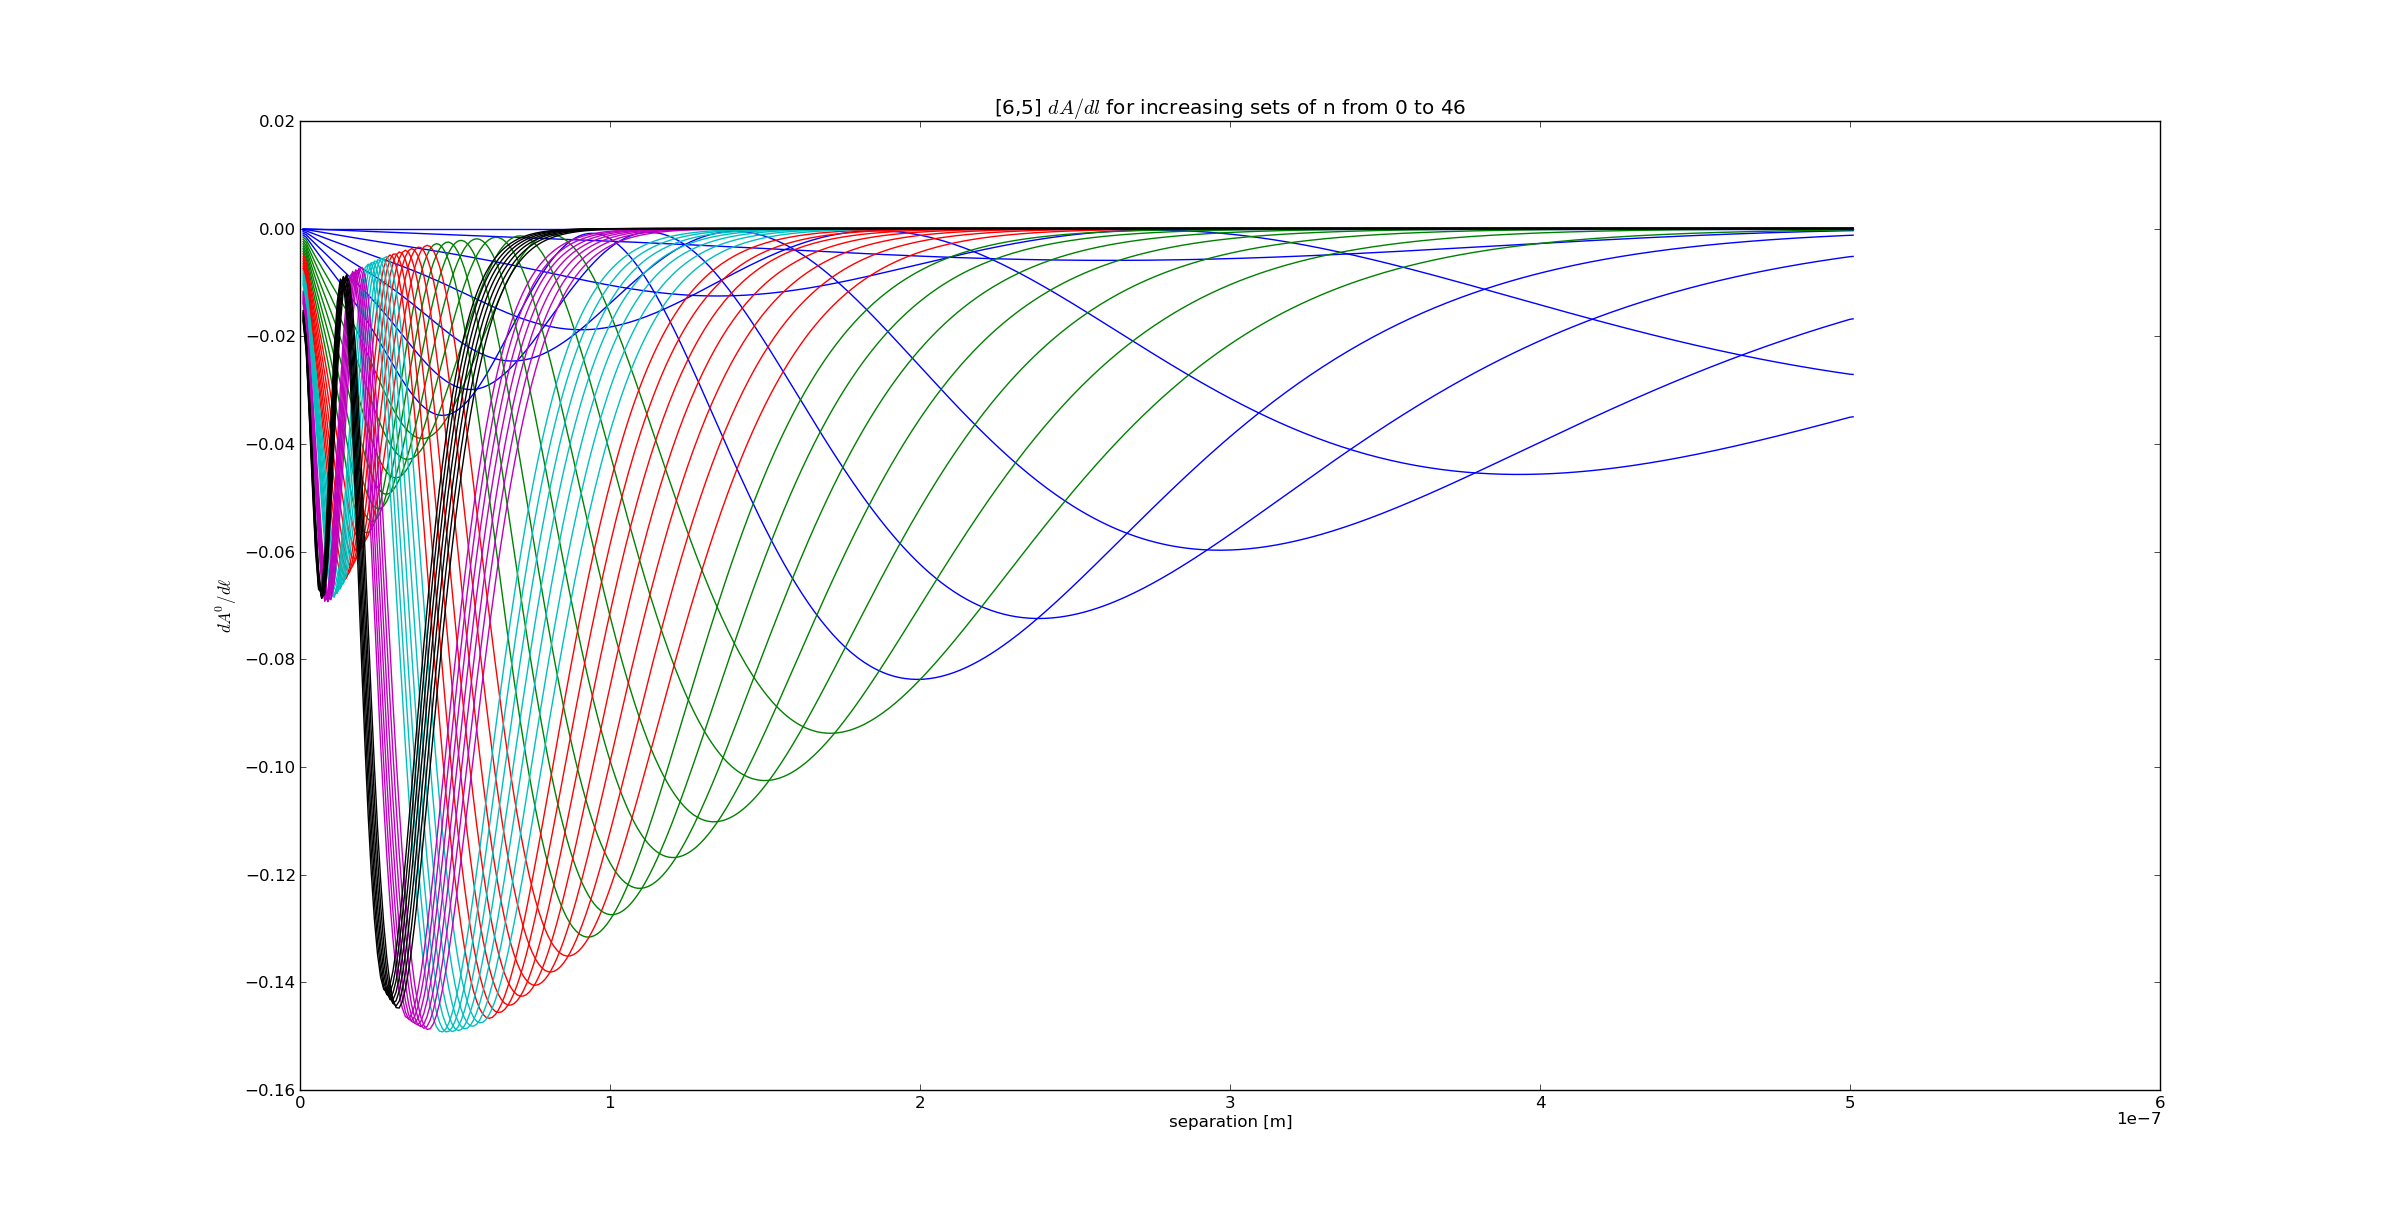
\includegraphics[width=1.2\textwidth,scale= 0.5]{plots/65_0to46.png}
\hskip 43pt
\caption{{\bf{The derivative of ${\cal A}^{(0)}$ with respect to separation for a
        range of values of n from n=0 to n=46.}} Derivative of Matsubara terms with 
        respect to $\ell$, $d{\cal A}^{(0)}/d\ell$, for two perpendicular [6,5] CNTs in water. 
        Colors represent groups of six increasing adjacent vales of n, i.e. for n=(0 to 6) blue, 
        n = (10 to 16) green, n = (20 to 26) red, and so on to n = (40 to 46) black.}
\label{eiz65}
\end{center}
\end{figure*} 

\hskip 73pt
%%%%%%%%%%%%%% 65 dA0/dl %%%%%%%%%%%%%%%%%%%%%%%%%%%%%%
\begin{figure*}[t!]
\begin{center}
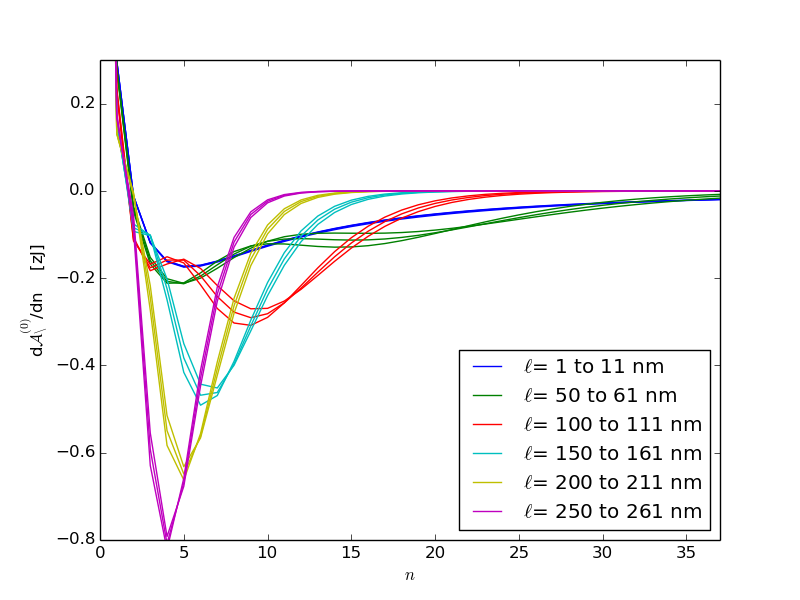
\includegraphics[width=1.2\textwidth,scale= 1.1]{plots/65_dAdn_vs_n.png}
\hskip 43pt
\caption{{\bf{The derivative of ${\cal A}^{(0)}$ with respect to n for different
    values of separation.}} Derivative of Matsubara terms with respect to n,
    $d{\cal A}^{(0)}/dn$, for two perpendicular [6,5] CNTs in water. Colors represent
groups of 3 values of $\ell$, i.e. blue for $\ell$= 1,6,11 nm, green for n =
50,56,61; red for $\ell$ = 100,106,111, and so on.}
\label{eiz65}
\end{center}
\end{figure*} 
\end{center}
%%%%%%%%%% [9,3] EPS2 and Aiz%%%%%%%%%%%%%%%%%%%%%%%%%%%%%%%%%%%%%%%%%%%%%%%%
%\section{CNT semi-metal [9,3]}
%\subsection{[9,3] dielectric response spectrum, dispersion spectrum, and anisotropy measure}
%\begin{center}
%From the imaginary part of the dielectric response function of the carbon
%nanotubes, we compute the London dispersion spectrum by the Kramers-Kronig
%transform:
%\begin{equation}
%\epsilon(i \zeta_n) = 1 + \frac{\pi}{2} \int_0^{\infty} dw
%~\frac{\epsilon\prime\prime(\omega)\omega}{\omega^{2} + \zeta^{2}}
%\end{equation}
%Where $\zeta_n = 2\pi n k_BT/\hbar$, and $n$ is an integer and the $n=0$ term is counted with a weight $1/2$. 
%
%Relative anisotropy measures in the parallel and perpendicular direction are given by
%\begin{equation}
%\Delta_{\perp}=\frac{{\epsilon^{c}}_{\perp}-\epsilon_{m}}{{\epsilon^{c}}_{\perp}+\epsilon_{m}}\qquad\Delta_{\parallel}=\frac{{\epsilon^{c}}_{\parallel}-\epsilon_{m}}{\epsilon_{m}}.
%\label{anisoind}
%\end{equation}
%
%Ratio of anisotropy measure:
%\begin{equation}
%a_{1,2}(i \omega_n) = \frac{2 \Delta_{\perp}^{(1,2)}(i\omega_n)}{\Delta_{\parallel}^{(1,2)}(i \omega_n)} = 
%2 \frac{({{\epsilon^{c}}_{\perp}}^{(1,2)}(i \omega_n) -\epsilon_{m}(i \omega_n)) \epsilon_{m}(i \omega_n)}{({{\epsilon^{c}}_{\perp}}^{(1,2)}(i \omega_n)+\epsilon_{m}(i \omega_n)) ({{\epsilon^{c}}_{\parallel}}^{(1,2)}(i \omega_n) -\epsilon_{m}(i \omega_n))}
%\label{eq:adef}
%\end{equation}
%
%\begin{figure*}[t!]
%\begin{center}
%\begin{minipage}[b]{0.40\textwidth}
%\begin{center}
%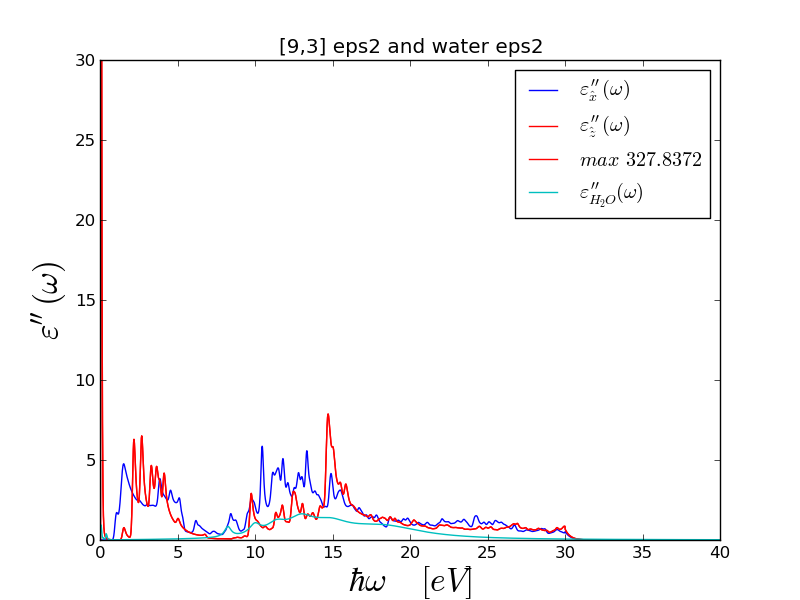
\includegraphics[width=1.4\textwidth]{prop_plots/93w93_eps2.png} (a)
%\end{center}
%\end{minipage}
%\hskip 43pt
%\begin{minipage}[b]{0.40\textwidth}
%\begin{center}
%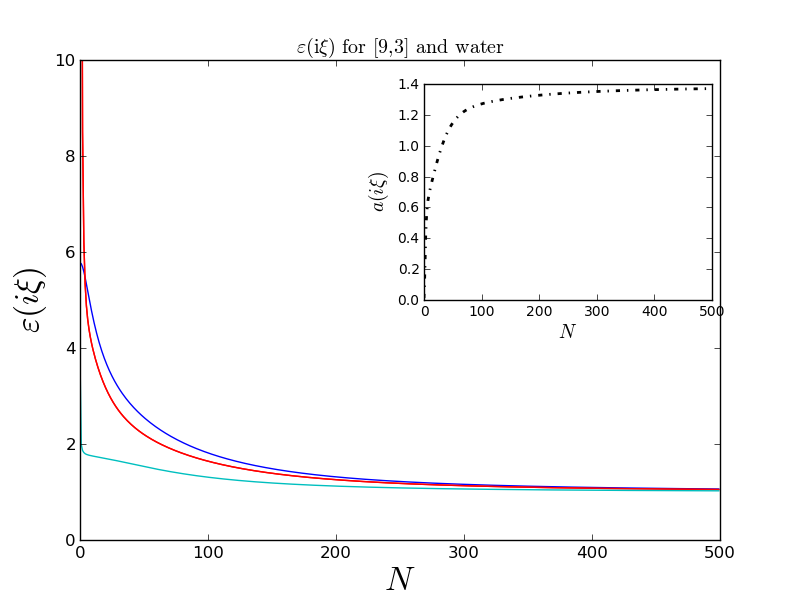
\includegraphics[width=1.4\textwidth]{prop_plots/93w93_eiz.png} (b)
%\end{center}
%\end{minipage}
%\caption{(a) Imaginary dielectric response spectrum, (b) dispersion spectrum and anistropy measure (inset)}
%\label{eiz91}
%\end{center}
%\end{figure*} 
%\end{center}
%\subsection{[9,3] dielectric contrast, anisotropy measure, and their derivatives}
%\begin{center}
%From the imaginary part of the dielectric response function of the carbon
%nanotubes, we compute the London dispersion spectrum by the Kramers-Kronig
%transform:
%\begin{equation}
%\epsilon(i \zeta_n) = 1 + \frac{\pi}{2} \int_0^{\infty} dw
%~\frac{\epsilon\prime\prime(\omega)\omega}{\omega^{2} + \zeta^{2}}
%\end{equation}
%Where $\zeta_n = 2\pi n k_BT/\hbar$, and $n$ is an integer and the $n=0$ term is counted with a weight $1/2$. 
%
%Relative anisotropy measures in the parallel and perpendicular direction are given by
%\begin{equation}
%\Delta_{\perp}=\frac{{\epsilon^{c}}_{\perp}-\epsilon_{m}}{{\epsilon^{c}}_{\perp}+\epsilon_{m}}\qquad\Delta_{\parallel}=\frac{{\epsilon^{c}}_{\parallel}-\epsilon_{m}}{\epsilon_{m}}.
%\label{anisoind}
%\end{equation}
%
%Ratio of anisotropy measure:
%\begin{equation}
%a_{1,2}(i \omega_n) = \frac{2 \Delta_{\perp}^{(1,2)}(i\omega_n)}{\Delta_{\parallel}^{(1,2)}(i \omega_n)} = 
%2 \frac{({{\epsilon^{c}}_{\perp}}^{(1,2)}(i \omega_n) -\epsilon_{m}(i \omega_n)) \epsilon_{m}(i \omega_n)}{({{\epsilon^{c}}_{\perp}}^{(1,2)}(i \omega_n)+\epsilon_{m}(i \omega_n)) ({{\epsilon^{c}}_{\parallel}}^{(1,2)}(i \omega_n) -\epsilon_{m}(i \omega_n))}
%\label{eq:adef}
%\end{equation}
%
%\begin{figure*}[t!]
%\begin{center}
%    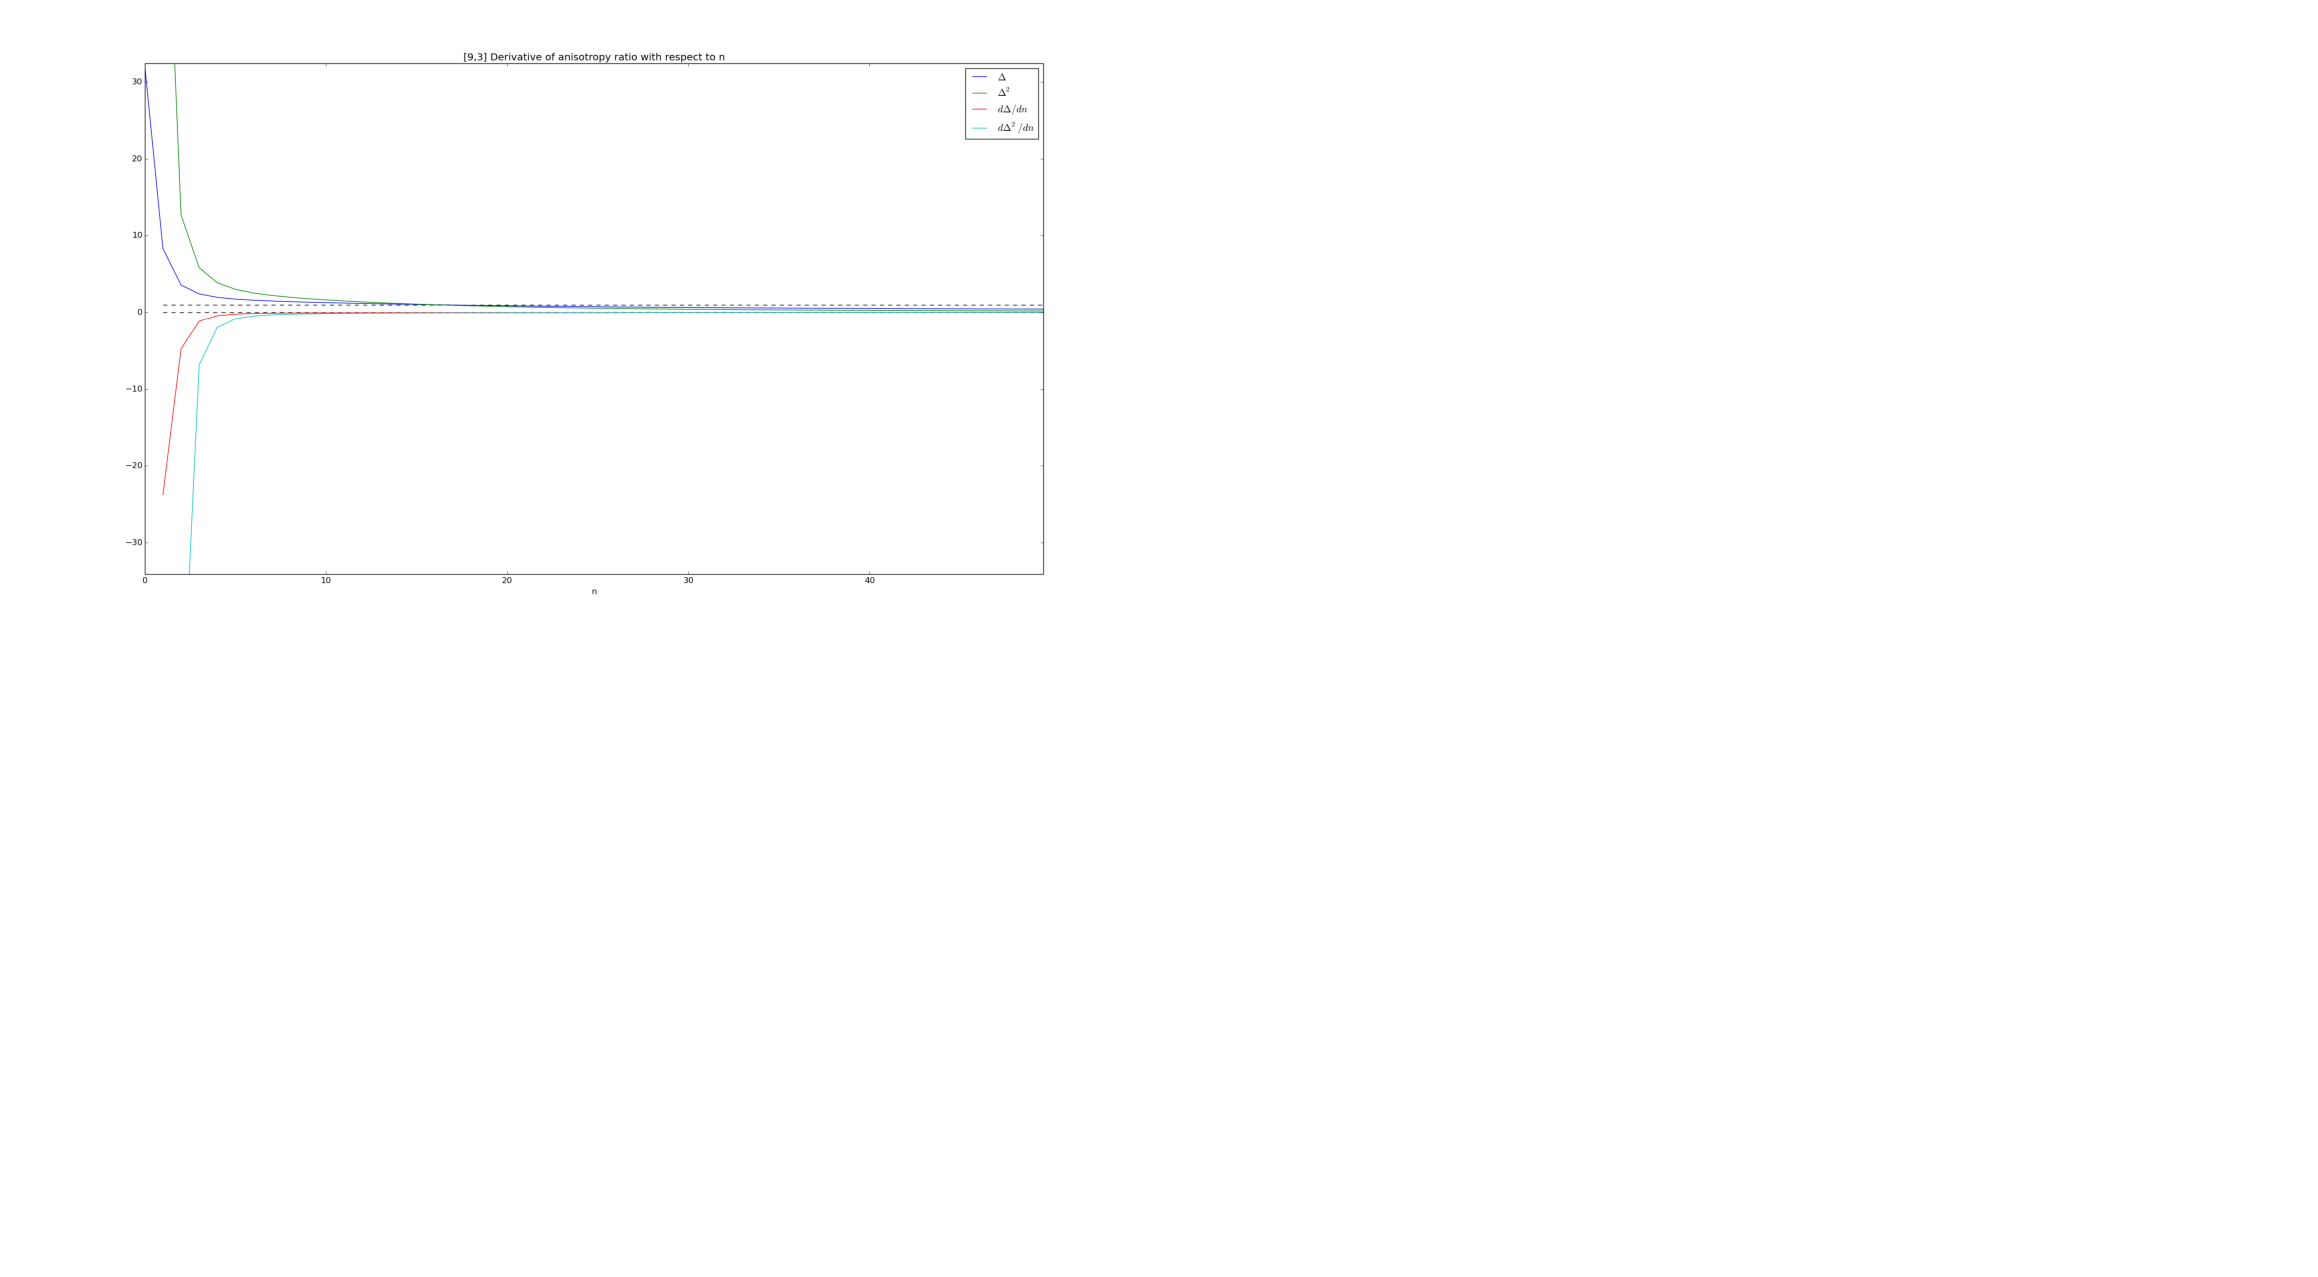
\includegraphics[width=1.2\textwidth]{plots/delta_derivs_93.png}
%\hskip 43pt
%\caption{Dielectric contrast of [9,3] CNTs in water, its square, and their
%derivatives with respect to n.} 
%\label{eiz65}
%\end{center}
%\end{figure*} 
%
%\begin{figure*}[t!]
%\begin{center}
%    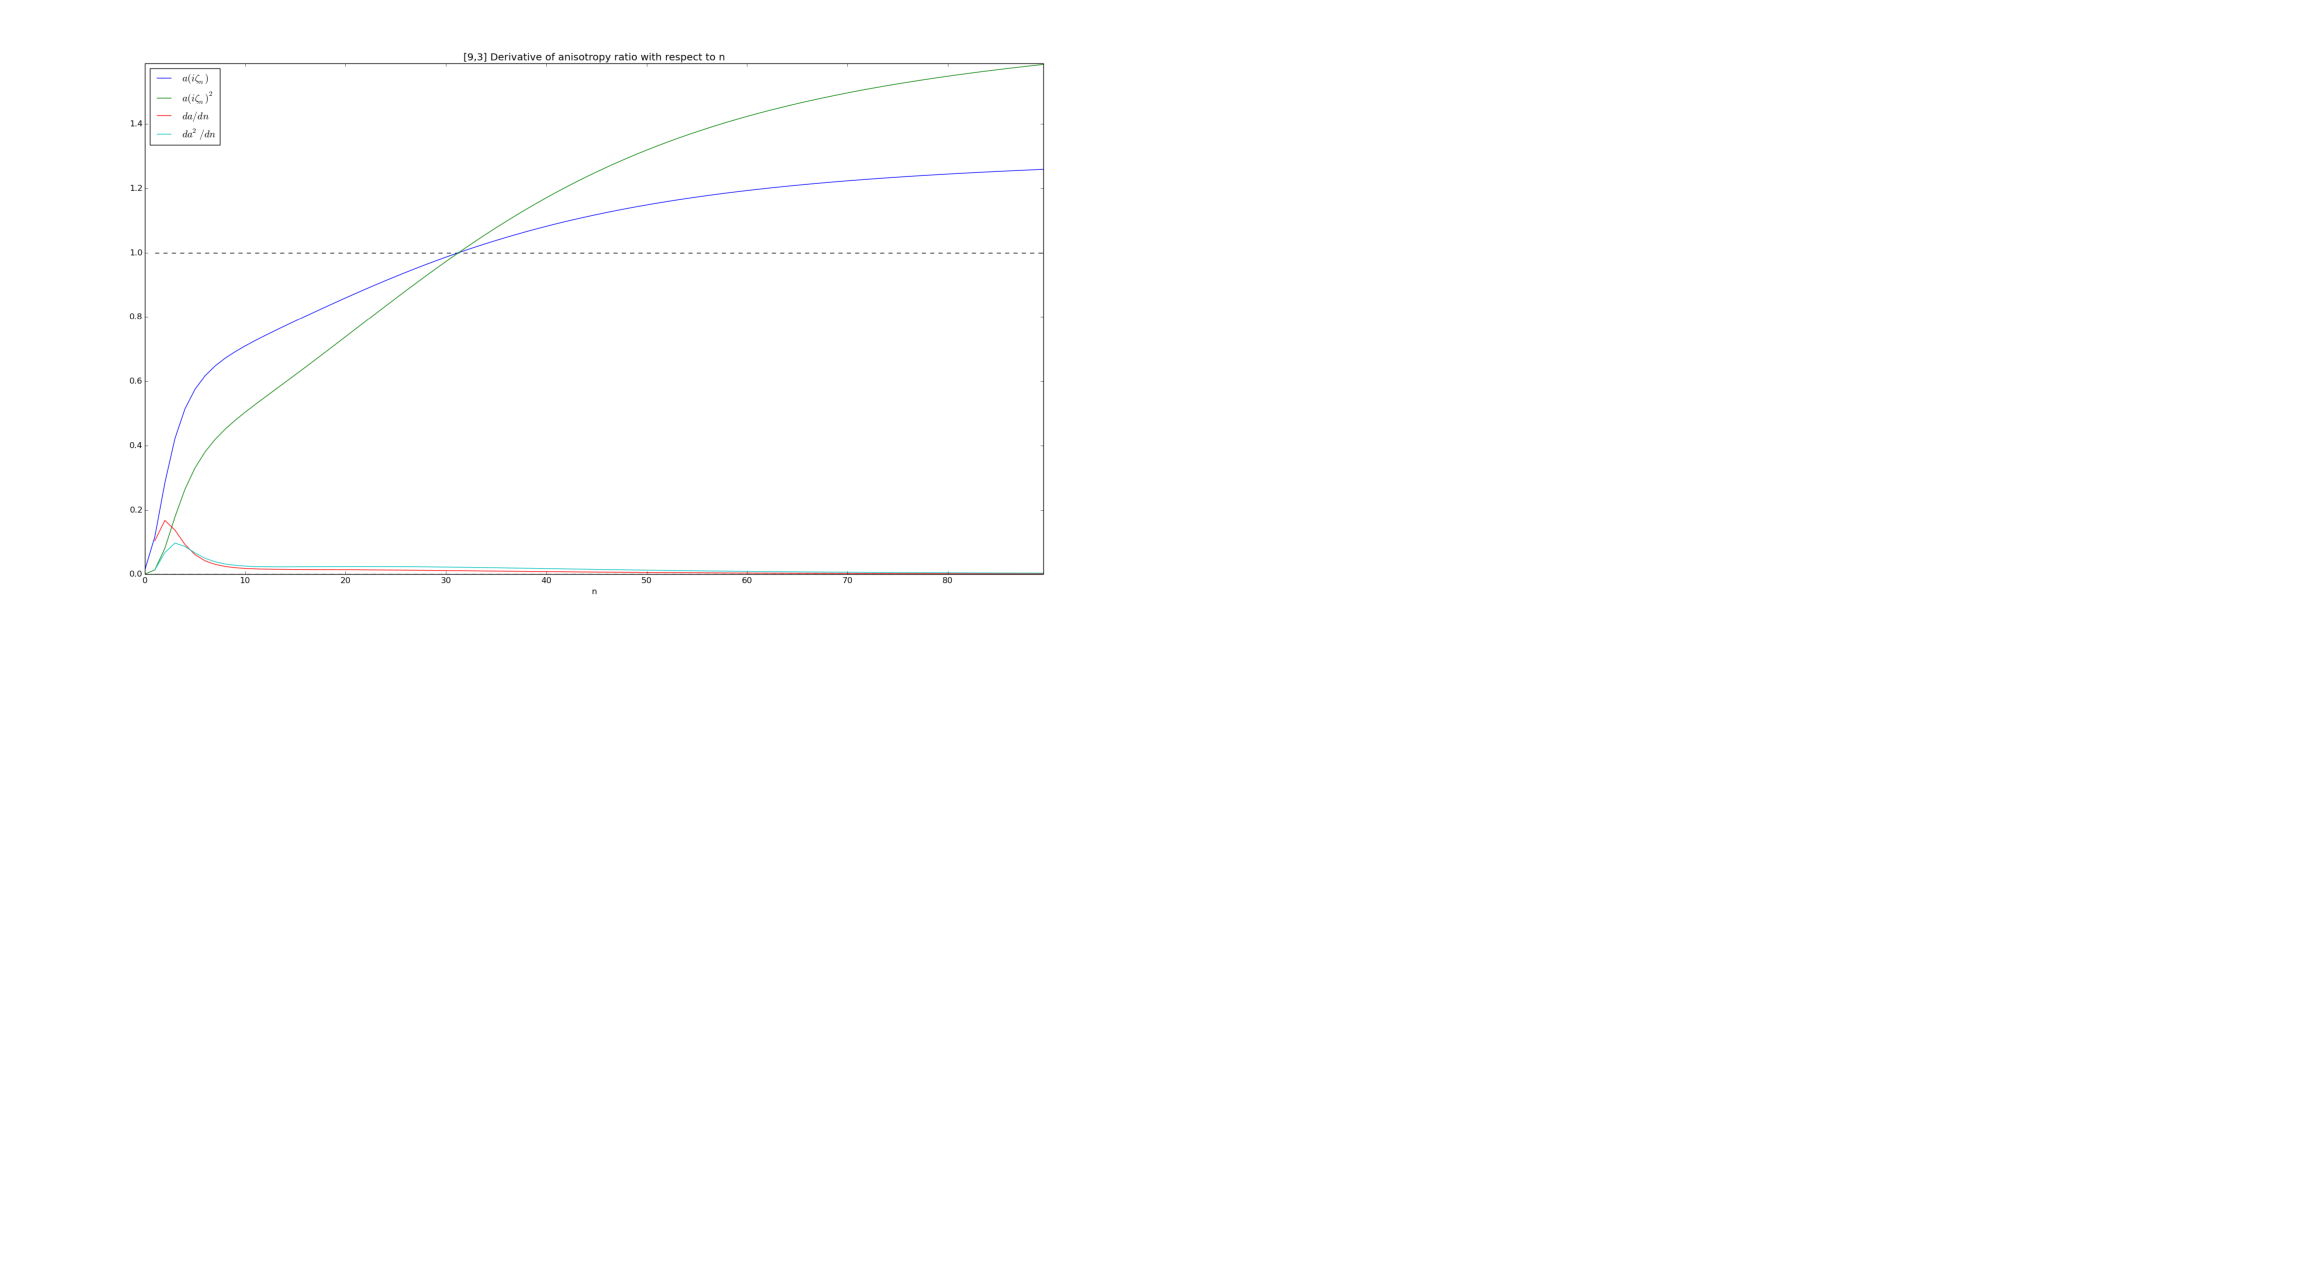
\includegraphics[width=1.2\textwidth]{plots/a_derivs_93.png}
%\hskip 43pt
%\caption{Anisotropy ratio of [9,3] CNTs in water, its square, and their
%derivatives with respect to n.} 
%\label{eiz65}
%\end{center}
%\end{figure*} 
%
%%%%%%%%%%%%%%%%%%%%%%%%%%%%%%%%%%[9,3] HAMAKERS %%%%%%%%%%%%%%%%%%%%%%%%%%%%%%%%
%\begin{center}
%\subsection{[9,3] Fully retarded Hamaker Coefficients for Matsubara Sum }
%%\subsection{[9,3] Log-log plot with $\cal{A}(n=0)=0$}
%\begin{equation}
%{\cal A}^{(0)}(\ell) = \frac{k_BT}{32}  {\sum_{n=0}^{\infty}}' \Delta_{1,\parallel} \Delta_{2,\parallel} ~p_n^{4}(\ell) ~\int_0^{\infty} t dt ~\frac{e^{- 2 p_n(\ell) \sqrt{t^{2} + 1}}}{(t^{2} + 1)} \tilde g^{(0)}(t, a_1(i \omega_n), a_2(i \omega_n))
%\end{equation}
%with
%\begin{multline*}
%%\begin{equation}
%%\begin{split}
%\tilde g^{(0)}(t, a_1(i \omega_n), a_2(i \omega_n)) = \\ 
%2 \left[ (1+3a_1)(1+3a_2) t^{4} + 2 (1+2a_1+2a_2+3a_1a_2) t^{2}  + 2(1+a_1)(1+a_2)\right]
%%\end{split}
%%\end{equation}
%\end{multline*}
%
%%\begin{equation}
%%\tilde g^{(0)}(t, a_1(i \omega_n), a_2(i \omega_n)) = 2 \left[ (1+3a_1)(1+3a_2) t^{4} + 2 (1+2a_1+2a_2+3a_1a_2) t^{2}  + 2(1+a_1)(1+a_2)\right]
%%\end{equation}
%and
%\begin{equation}
%{\cal A}^{(2)}(\ell) = \frac{k_BT}{32}  {\sum_{n=0}^{\infty}}' \Delta_{1,\parallel} \Delta_{2,\parallel} ~p_n^{4}(\ell) ~\int_0^{\infty} t dt ~\frac{e^{- 2 p_n(\ell) \sqrt{t^{2} + 1}}}{(t^{2} + 1)} \tilde g^{(2)}(t, a_1(i \omega_n), a_2(i \omega_n), \theta)
%\end{equation}
%with
%\begin{equation}
%\tilde g^{(2)}(t, a_1(i \omega_n), a_2(i \omega_n), \theta) = (1-a_1)(1-a_2)(t^{2} + 2)^2
%\label{befgqw}
%\end{equation}
%
%\begin{figure*}[t!]
%\begin{center}
%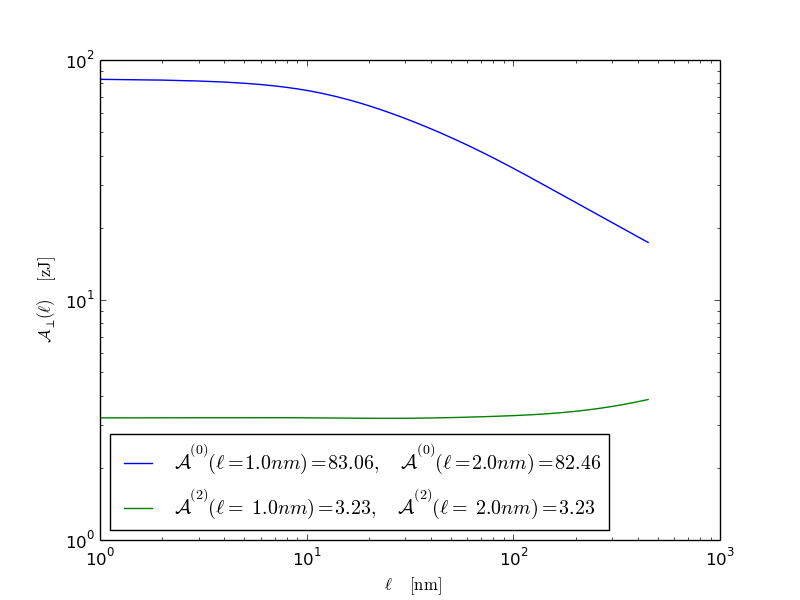
\includegraphics[width=1.0\textwidth]{plots/140322_93w93_HCs_n0_equal_0_perpendicular_ret.png}
%\hskip 43pt
%\caption{Full result}
%\label{eiz65}
%\end{center}
%\end{figure*}
%
%%%%%%%%%%%%%%%%%%%%%%%%%%%%%%%%%% [9,3] SEMILOG A %%%%%%%%%%%%%%%%
%%\subsection{[9,3] Semi-log plot with $\cal{A}(n=0)=0$}
%\begin{figure*}[t!]
%\begin{center}
%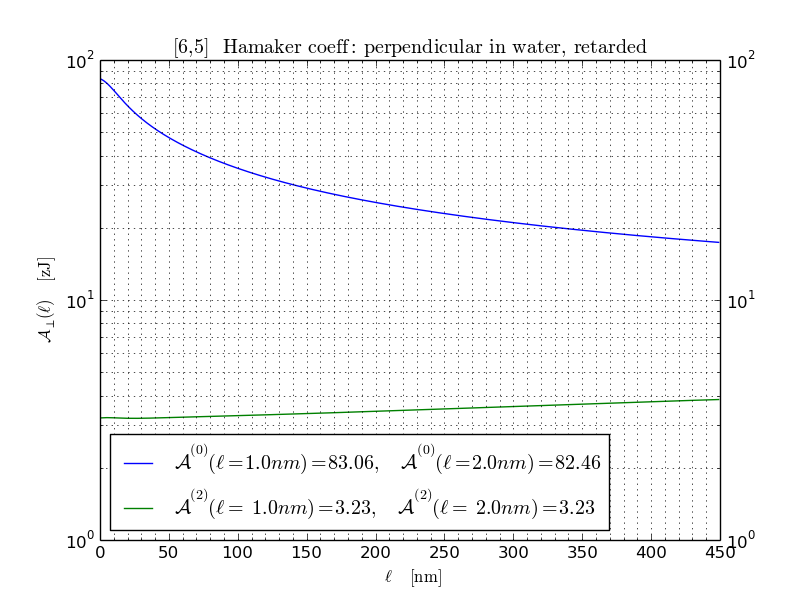
\includegraphics[width=1.0\textwidth]{plots/140322_93w93_HCs_n0_equal_0_semilog_perpendicular_ret.png}
%\hskip 43pt
%\caption{Full result}
%\label{eiz65}
%\end{center}
%\end{figure*} 
%
%\end{center}
%
%%%%%%%%%%%%%%%%%%%%%%%%%%%%%%%%%% [9,3] Terms A %%%%%%%%%%%%%%%%
%\subsection{[9,3] Terms of Matsubara sum with $\cal{A}(n=0)=0$}
%\begin{center}
%We write the Hamaker coefficients as,
%\begin{equation}
%{\cal A}^{(0)}(\ell) = \frac{k_BT}{32}  {\sum_{n=0}^{\infty}}' \Delta_{1,\parallel} \Delta_{2,\parallel} ~p_n^{4}(\ell) ~\int_0^{\infty} t dt ~\frac{e^{- 2 p_n(\ell) \sqrt{t^{2} + 1}}}{(t^{2} + 1)} \tilde g^{(0)}(t, a_1(i \omega_n), a_2(i \omega_n))
%\end{equation}
%with
%\begin{multline*}
%\tilde g^{(0)}(t, a_1(i \omega_n), a_2(i \omega_n)) = \\ 
%2 \left[ (1+3a_1)(1+3a_2) t^{4} + 2 (1+2a_1+2a_2+3a_1a_2) t^{2}  + 2(1+a_1)(1+a_2)\right]
%\end{multline*}
%and
%\begin{equation}
%{\cal A}^{(2)}(\ell) = \frac{k_BT}{32}  {\sum_{n=0}^{\infty}}' \Delta_{1,\parallel} \Delta_{2,\parallel} ~p_n^{4}(\ell) ~\int_0^{\infty} t dt ~\frac{e^{- 2 p_n(\ell) \sqrt{t^{2} + 1}}}{(t^{2} + 1)} \tilde g^{(2)}(t, a_1(i \omega_n), a_2(i \omega_n), \theta)
%\end{equation}
%with
%\begin{equation*}
%\tilde g^{(2)}(t, a_1(i \omega_n), a_2(i \omega_n), \theta) = (1-a_1)(1-a_2)(t^{2} + 2)^2
%\label{befgqw}
%\end{equation*}
%Where
%\begin{equation*}
%p_n^{2}(\ell) =  \epsilon_m(i \omega_n) \frac{\omega_n^{2}}{c^{2}} \ell^{2},
%\end{equation*}
%\begin{equation*}
%\Delta_{\perp}=\frac{{\epsilon^{c}}_{\perp}-\epsilon_{m}}{{\epsilon^{c}}_{\perp}+\epsilon_{m}}\qquad\Delta_{\parallel}=\frac{{\epsilon^{c}}_{\parallel}-\epsilon_{m}}{\epsilon_{m}},
%\label{anisoind}
%\end{equation*}
%\begin{equation*}
%a = \frac{2 \Delta_{\perp}}{\Delta_{\parallel}} = 2 \frac{({\epsilon^{c}}_{\perp}-\epsilon_{m}) \epsilon_{m}}{({\epsilon^{c}}_{\perp}+\epsilon_{m}) ({\epsilon^{c}}_{\parallel}-\epsilon_{m})}
%\label{eq:adef}
%\end{equation*}
%
%For n = 0, we use
%\begin{equation}
%    {\cal A}_{n=0}^{(0)}(\ell) = \frac{1}{2} \frac{k_BT}{32}
%    \Delta_{1,\parallel} \Delta_{2,\parallel} ~\int_0^{\infty} u^3 du\,\,
%    e^{-2u}\,\,[2(1 + 3a_1)(1 + 3a_2) ]
%\end{equation}
%and
%\begin{equation}
%    {\cal A}_{n=0}^{(2)}(\ell) = \frac{1}{2} \frac{k_BT}{32}
%    \Delta_{1,\parallel} \Delta_{2,\parallel} ~\int_0^{\infty} u^3 du\,\,
%    e^{-2u}\,\,[(1 - a_1)(1 - a_2) ]
%\end{equation}
%where $u = Ql$.
%
%\begin{equation}
%{\cal A}^{(0)}(\ell) = \frac{k_BT}{32}  {\sum_{n=0}^{\infty}}' \Delta_{1,\parallel} \Delta_{2,\parallel} ~p_n^{4}(\ell) ~\int_0^{\infty} t dt ~\frac{e^{- 2 p_n(\ell) \sqrt{t^{2} + 1}}}{(t^{2} + 1)} \tilde g^{(0)}(t, a_1(i \omega_n), a_2(i \omega_n))
%\end{equation}
%with
%\begin{equation}
%\tilde g^{(0)}(t, a_1(i \omega_n), a_2(i \omega_n)) = 2 \left[ (1+3a_1)(1+3a_2) t^{4} + 2 (1+2a_1+2a_2+3a_1a_2) t^{2}  + 2(1+a_1)(1+a_2)\right]
%\end{equation}
%and
%\begin{equation}
%{\cal A}^{(2)}(\ell) = \frac{k_BT}{32}  {\sum_{n=0}^{\infty}}' \Delta_{1,\parallel} \Delta_{2,\parallel} ~p_n^{4}(\ell) ~\int_0^{\infty} t dt ~\frac{e^{- 2 p_n(\ell) \sqrt{t^{2} + 1}}}{(t^{2} + 1)} \tilde g^{(2)}(t, a_1(i \omega_n), a_2(i \omega_n), \theta)
%\end{equation}
%with
%\begin{equation}
%\tilde g^{(2)}(t, a_1(i \omega_n), a_2(i \omega_n), \theta) = (1-a_1)(1-a_2)(t^{2} + 2)^2
%\label{befgqw}
%\end{equation}
%
%\begin{figure*}[t!]
%\begin{center}
%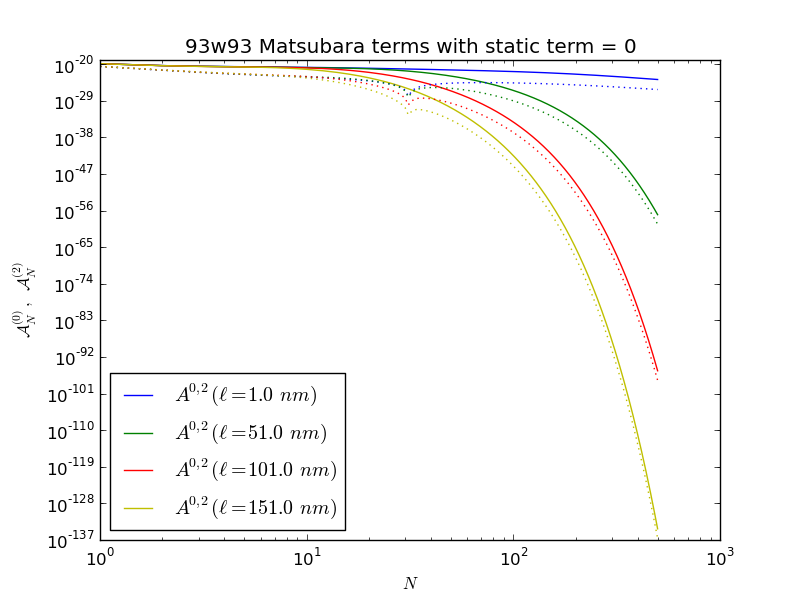
\includegraphics[width=1.0\textwidth]{plots/93_n0_A_vs_n.png}
%\hskip 43pt
%\caption{Full result}
%\label{eiz65}
%\end{center}
%\end{figure*} 
%
%
%%%%%%%%%%%%%%% 93 dA0/dl %%%%%%%%%%%%%%%%%%%%%%%%%%%%%%
%\begin{figure*}[t!]
%\begin{center}
%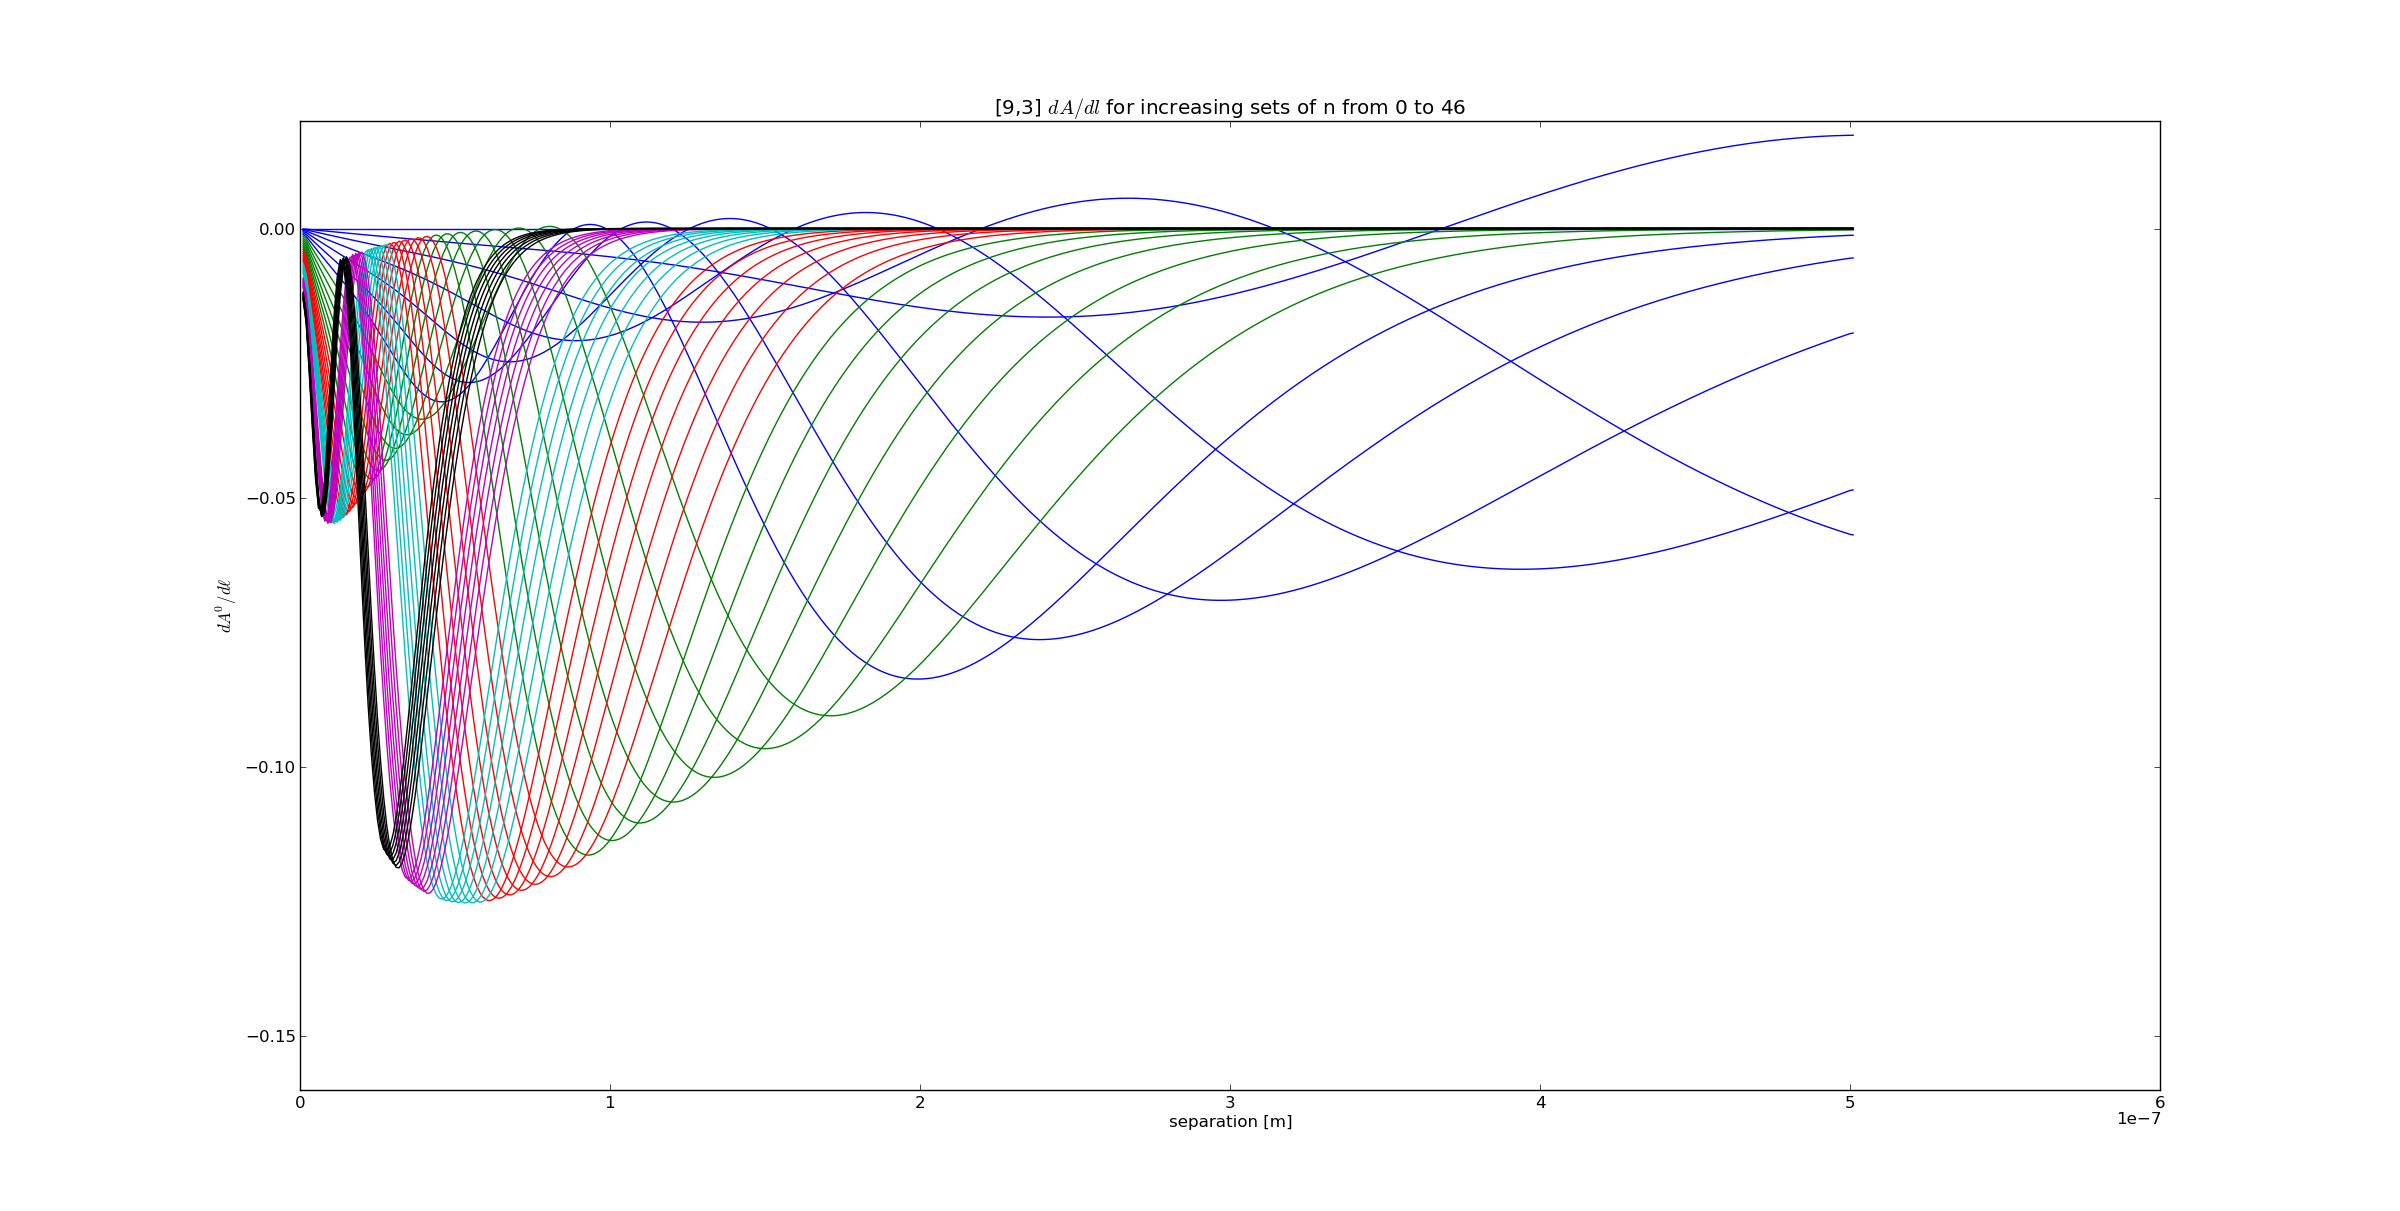
\includegraphics[width=1.2\textwidth]{plots/93_0to46.png}
%\hskip 43pt
%\caption{Derivative of Matsubara terms with respect to $\ell$,
%    $d\cal{A}^(0)/d\ell$, for two perpendicular [9,3] CNTs in water. Colors represent
%groups of six increasing adjacent vales of n, i.e. for n=(0 to 6) blue, n = (10
%to 16) green, n = (20 to 26) red, and so on to n = (40 to 46) black.}
%\label{eiz65}
%\end{center}
%\end{figure*} 
%
%\end{center}
%











%%%%%%%%%%%%%%%%%%%%%%%%%%%%%%%%%A0 and A2 plot FOR KINK in [9,3] A0 %%%%%%%%%%%
\section{Finite c effect: change in contributions to Matsubara sum of
${\cal A}^{(0)}$}
\subsection{[6,5] as an example of power law knee in ${\cal A}^{(0)}$ and
    inflection points in $d {\cal A}^{(0)} / \it{d}\ell$}
%\subsection{Plot of $\cal{A}^{(0)}$ and $\cal{A}^{(2)}$ for [9,3]}
\begin{center}
\begin{equation}
{\cal A}^{(0)}(\ell) = \frac{k_BT}{32}  {\sum_{n=0}^{\infty}}' \Delta_{1,\parallel} \Delta_{2,\parallel} ~p_n^{4}(\ell) ~\int_0^{\infty} t dt ~\frac{e^{- 2 p_n(\ell) \sqrt{t^{2} + 1}}}{(t^{2} + 1)} \tilde g^{(0)}(t, a_1(i \omega_n), a_2(i \omega_n))
\end{equation}
with
\begin{multline*}
%\begin{equation}
%\begin{split}
\tilde g^{(0)}(t, a_1(i \omega_n), a_2(i \omega_n)) = \\ 
2 \left[ (1+3a_1)(1+3a_2) t^{4} + 2 (1+2a_1+2a_2+3a_1a_2) t^{2}  + 2(1+a_1)(1+a_2)\right]
%\end{split}
%\end{equation}
\end{multline*}
%\begin{equation}
%\tilde g^{(0)}(t, a_1(i \omega_n), a_2(i \omega_n)) = 2 \left[ (1+3a_1)(1+3a_2) t^{4} + 2 (1+2a_1+2a_2+3a_1a_2) t^{2}  + 2(1+a_1)(1+a_2)\right]
%\end{equation}
and
\begin{equation}
{\cal A}^{(2)}(\ell) = \frac{k_BT}{32}  {\sum_{n=0}^{\infty}}' \Delta_{1,\parallel} \Delta_{2,\parallel} ~p_n^{4}(\ell) ~\int_0^{\infty} t dt ~\frac{e^{- 2 p_n(\ell) \sqrt{t^{2} + 1}}}{(t^{2} + 1)} \tilde g^{(2)}(t, a_1(i \omega_n), a_2(i \omega_n), \theta)
\end{equation}
with
\begin{equation}
\tilde g^{(2)}(t, a_1(i \omega_n), a_2(i \omega_n), \theta) = (1-a_1)(1-a_2)(t^{2} + 2)^2
\label{befgqw}
\end{equation}

%%%%%%%%%%%% Example plot of [6,5] A0 and A2 %%%%%%%%%%%%%%%
\begin{figure*}[t!]
\begin{center}
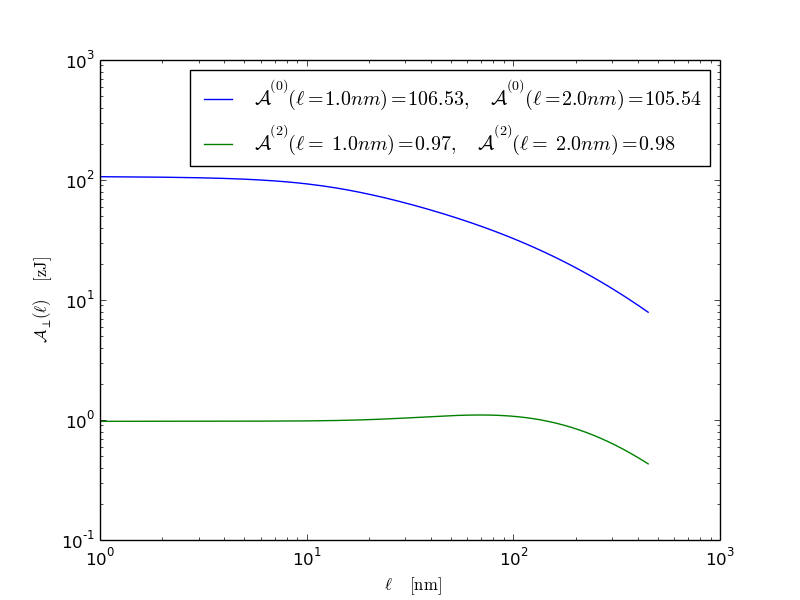
\includegraphics[width=1.2\textwidth]{plots/140322_65w65_HCs_perpendicular_ret.png}
%    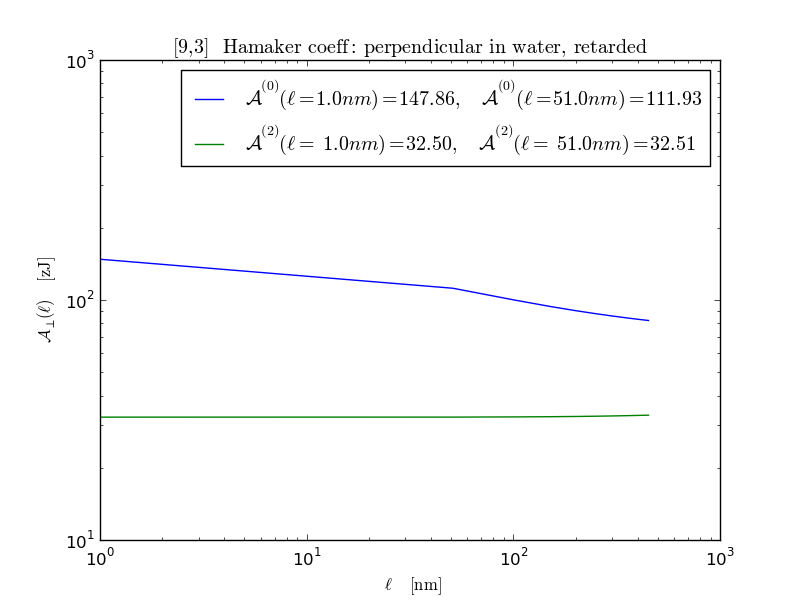
\includegraphics[width=1.2\textwidth]{plots/140322_93w93_HCs_perpendicular_ret.png}
\hskip 43pt
\caption{{\bf ${\cal A}^{(0,2)}$ as a function of separation for identical [6,5]
    CNTs in water.} For some separation, $\ell$, the function ${\cal A}^{(0)}$
displays a knee due to a changge in power law.}
\label{eiz65}
\end{center}
\end{figure*} 

%%%%%%%%%%%%%% d/dl of sumA0 vs n for 3 n's %%%%%%%%%%%%%%%%%%%%%%%%%%%%%%
\hskip 73pt

\begin{figure*}[t!]
\begin{center}
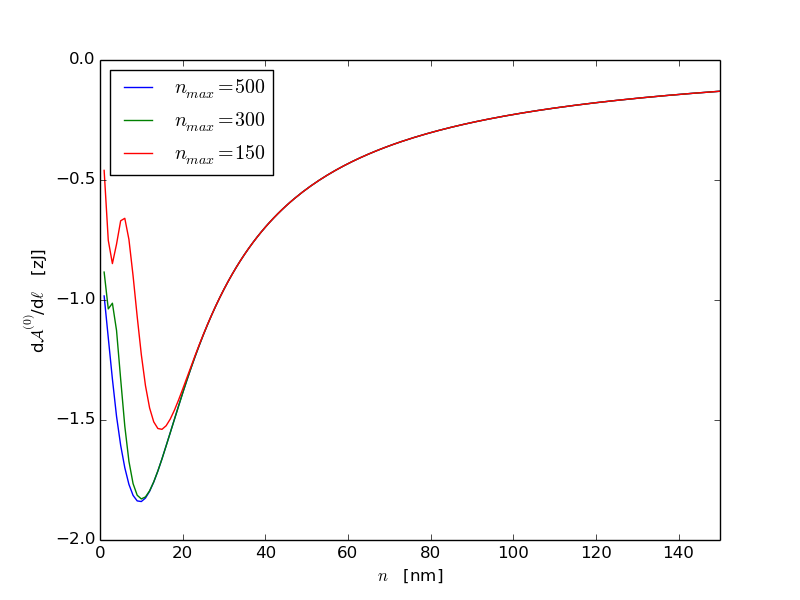
\includegraphics[width=1.2\textwidth]{plots/65_dsumAdl_vs_n.png}
\hskip 43pt
\caption{{\bf Derivative of ${\cal A}^{(0)} = \sum{\cal A}_n^{(0)}$ as a function of separation for
Matsubara sums to n=500,300, and 150.}  For typical calculations of this type
of CNT, sums from n=0 to n=500 are sufficient to capture n-dependant behavior
and are accurate to about 0.01 percent of sums to
n=10,000.  I use an upper limit of n = 500 for my computations, shown in blue. A
knee occurs in ${\cal A}^{(0)}(\ell)$ at the separation value for which
$\it{d}{\cal A}^{(0)}/\it{d}\ell \approx$0.  However, some of my other calculations
have indicated the existance of two inflection points at low values of $n$ and
$\ell$ in $\partial{\cal A}^{(0)}/\partial\ell$ as well as in
$\partial{\cal A}^{(0)}/\partial n$.
It appears that summing over the n's has the effect of blurring the two
inflection points into one inflection point.  The plot shows
the derivative of ${\cal A}^{(0)}$ with respect to separation with n=500 (blue),
n= 300 (green), and n=150 (red) used as the upper limit of the Matsubara sum.
When higher values of n are removed from the sum, their effect of merging the two
inflection points is also removed, as seen in green in red. }
\label{eiz65}
\end{center}
\end{figure*} 

\hskip 73pt
\end{center}

\subsection{Ratio of signal travel time to flucuation lifetime}%etardation factor $p_n(\ell)$}
Round-trip distance between correlated charge fluctuations: $2\ell$//
Round-trip travel time: $(2\ell)/(c/\sqrt{\epsilon_m})$ //
Fluctuation lifetime = $1/\zeta_n$//
Ratio $r_n$ = travel time/flucuation lifetime = $2\ell \sqrt{\epsilon_m}
\zeta_n/ c$ = (1/2)$p_n(\ell)$ from RP's report//

%%%%%%%%%%%%%%%%%%%%%%%%%%%%PLOT OF p(n,l)%%%%%%%%%%%%%%%%%%
\begin{center}
\begin{equation}
{\cal A}^{(0)}(\ell) = \frac{k_BT}{32}  {\sum_{n=0}^{\infty}}' \Delta_{1,\parallel} \Delta_{2,\parallel} ~p_n^{4}(\ell) ~\int_0^{\infty} t dt ~\frac{e^{- 2 p_n(\ell) \sqrt{t^{2} + 1}}}{(t^{2} + 1)} \tilde g^{(0)}(t, a_1(i \omega_n), a_2(i \omega_n))
\end{equation}
\begin{equation}
\tilde g^{(0)}(t, a_1(i \omega_n), a_2(i \omega_n)) = 2 \left[ (1+3a_1)(1+3a_2) t^{4} + 2 (1+2a_1+2a_2+3a_1a_2) t^{2}  + 2(1+a_1)(1+a_2)\right]
\end{equation}
and
\begin{equation}
{\cal A}^{(2)}(\ell) = \frac{k_BT}{32}  {\sum_{n=0}^{\infty}}' \Delta_{1,\parallel} \Delta_{2,\parallel} ~p_n^{4}(\ell) ~\int_0^{\infty} t dt ~\frac{e^{- 2 p_n(\ell) \sqrt{t^{2} + 1}}}{(t^{2} + 1)} \tilde g^{(2)}(t, a_1(i \omega_n), a_2(i \omega_n), \theta)
\end{equation}
with
\begin{equation}
\tilde g^{(2)}(t, a_1(i \omega_n), a_2(i \omega_n), \theta) = (1-a_1)(1-a_2)(t^{2} + 2)^2
\label{befgqw}
\end{equation}

where $p_n^{2}(\ell) =  \epsilon_m(i \omega_n) \frac{\omega_n^{2}}{c^{2}}
\ell^{2}$. \\

with the n = 0 term given by
\begin{equation}
    {\cal A}_{n=0}^{(0)}(\ell) = \frac{1}{2} \frac{k_BT}{32}
    \Delta_{1,\parallel} \Delta_{2,\parallel} ~\int_0^{\infty} u^3 du\,\,
    e^{-2u}\,\,[2(1 + 3a_1)(1 + 3a_2) ]
\end{equation}
and
\begin{equation}
    {\cal A}_{n=0}^{(2)}(\ell) = \frac{1}{2} \frac{k_BT}{32}
    \Delta_{1,\parallel} \Delta_{2,\parallel} ~\int_0^{\infty} u^3 du\,\,
    e^{-2u}\,\,[(1 - a_1)(1 - a_2) ]
\end{equation}
where $u = Ql$.



%%%%%%%%%%%%%% p vs l and pvs n %%%%%%%%%%%%%%%%%%%%%%%%%%%%%%
\hskip 73pt

\begin{figure*}[t!]
\begin{center}
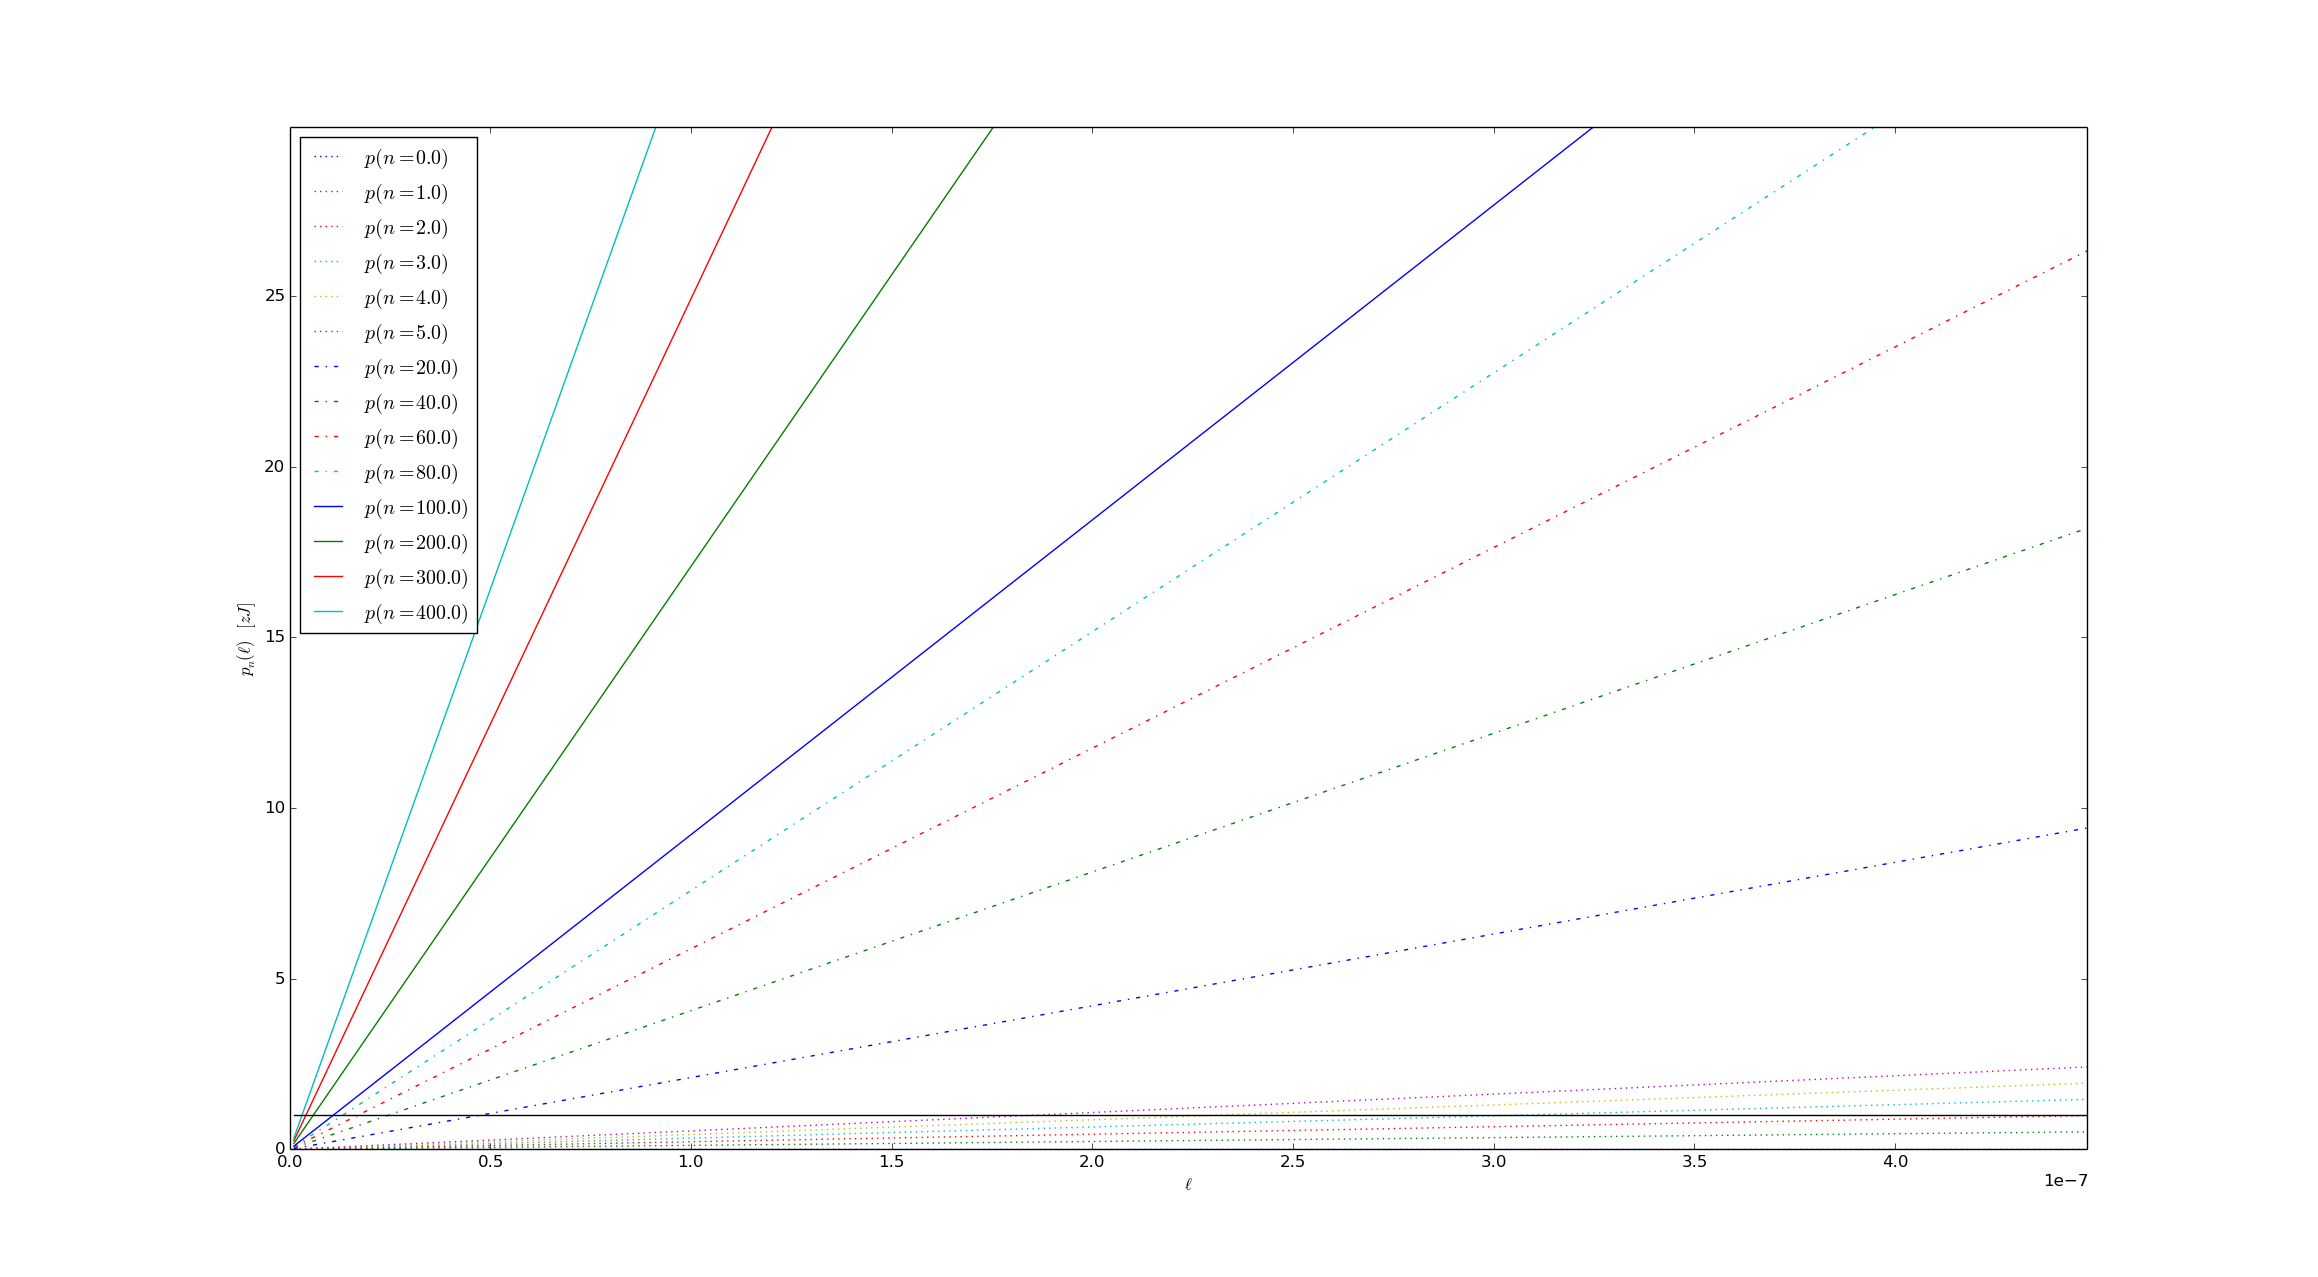
\includegraphics[width=1.2\textwidth,scale=0.5]{plots/pn_vs_l.png}
\hskip 43pt
\caption{{\bf $p_n(\ell)$ vs $\ell$} for several values of n, where $p_n^{2}(\ell) =  \epsilon_m(i \omega_n) \frac{\omega_n^{2}}{c^{2}} \ell^{2}$. .  For each value of n (corresponding to different line colors and line styles), there is an $\ell$ value for which $p_n(\ell)=1$.  A black line is provided to show $p_n=1$.}
\label{eiz65}
\end{center}
\end{figure*} 
\hskip 73pt

\begin{figure*}[t!]
\begin{center}
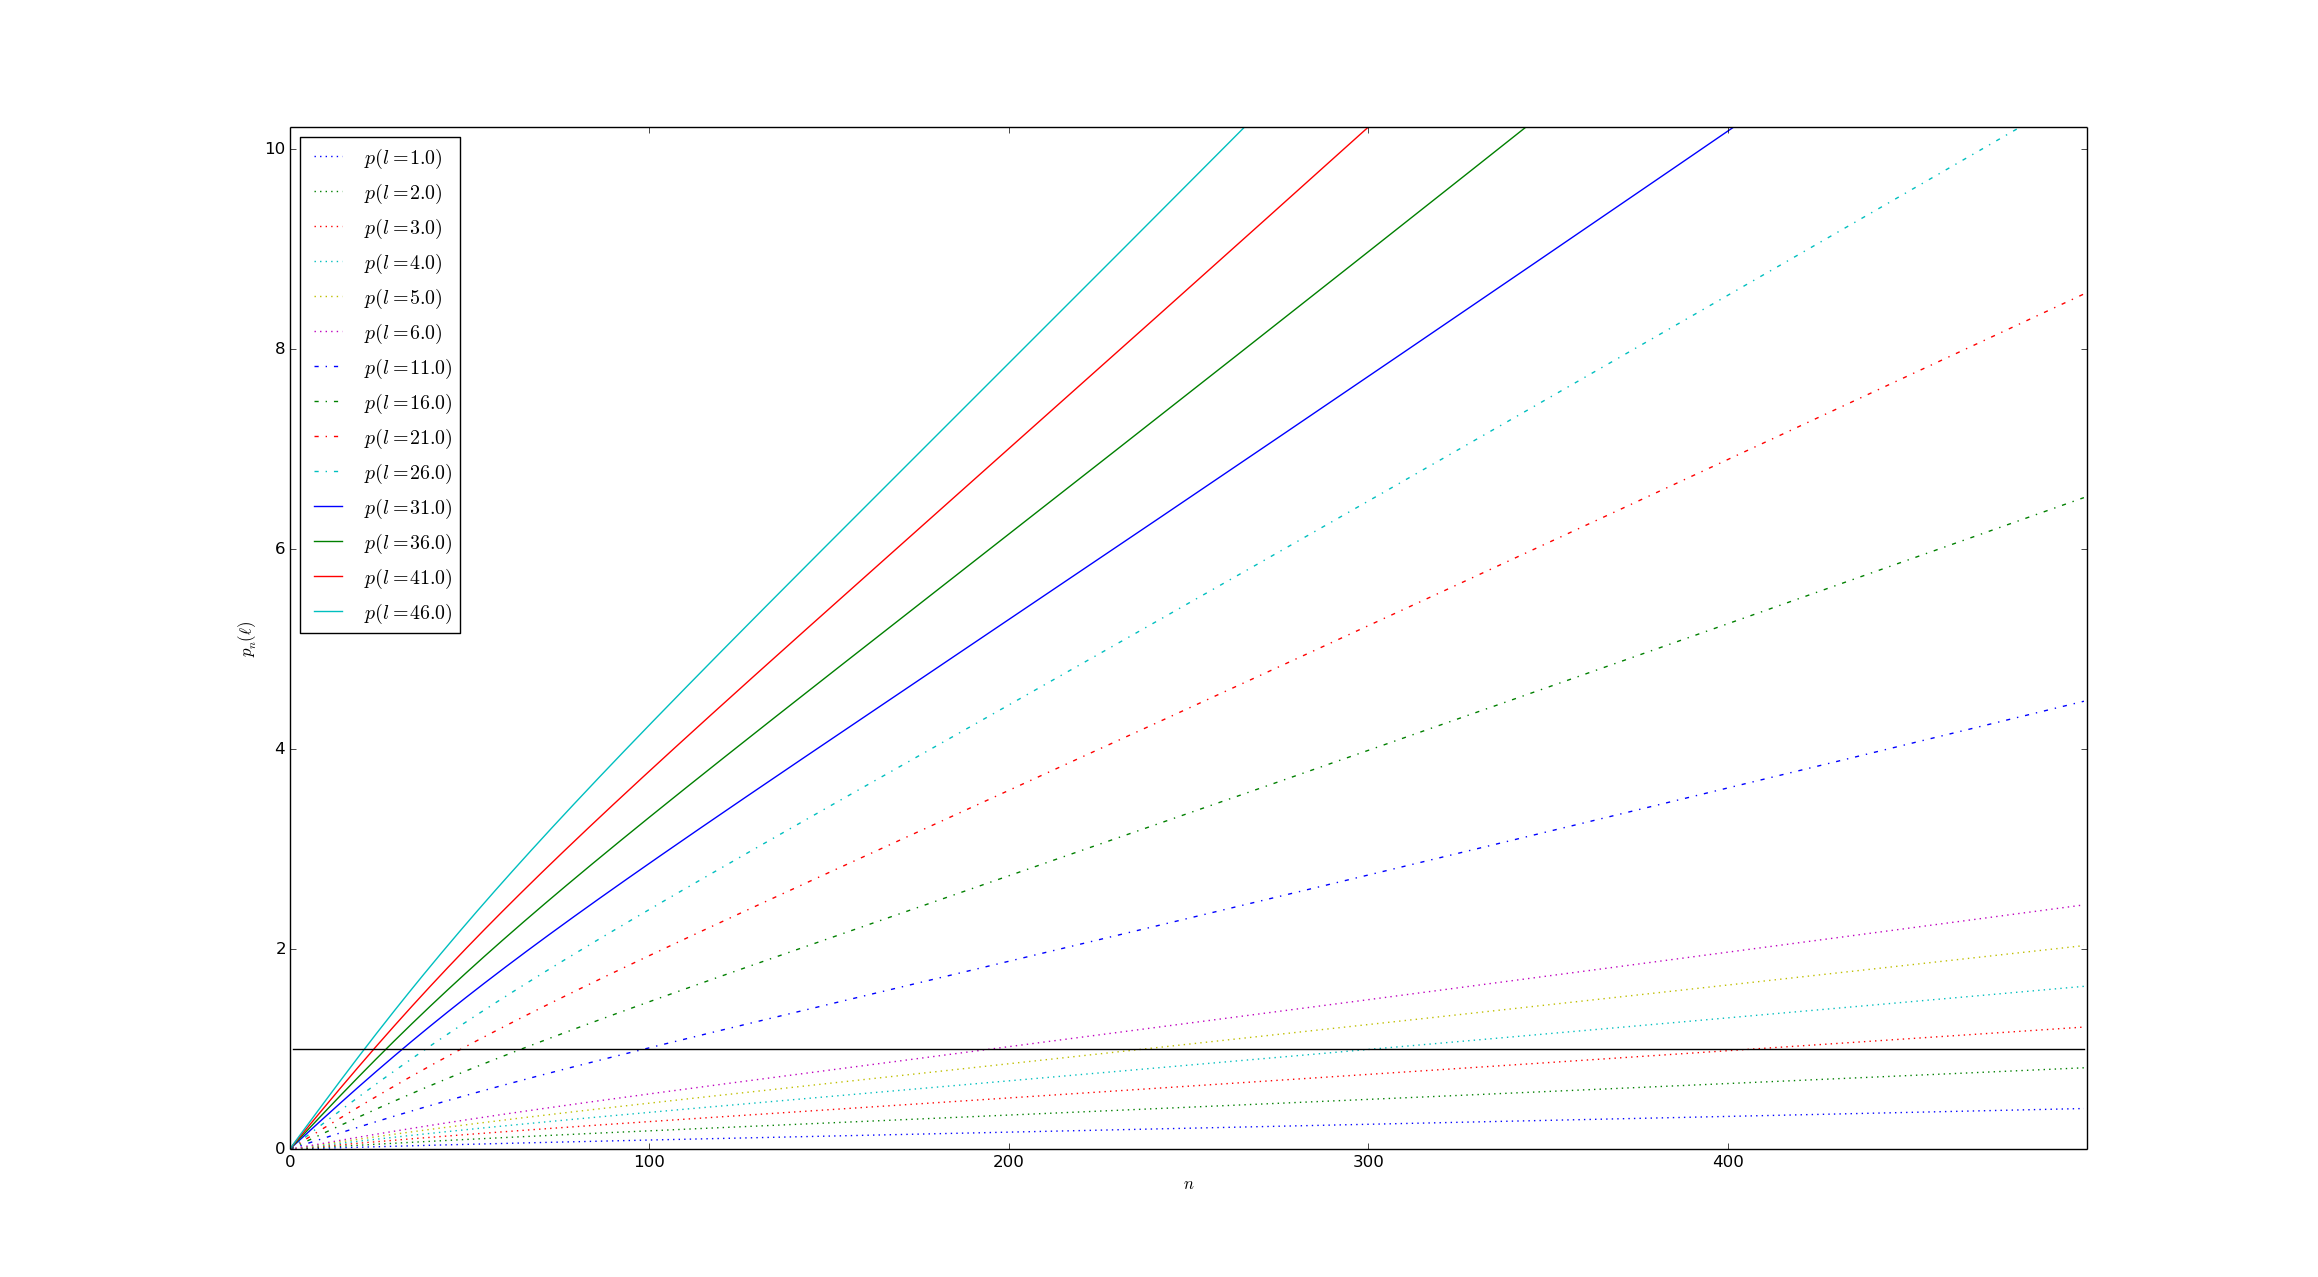
\includegraphics[width=1.2\textwidth,scale=0.5]{plots/pn_vs_n.png}
\hskip 43pt
\caption{{\bf $p_n(\ell)$ vs $n$} for several values of $\ell$.  For each value of
    $\ell$ (corresponding to different line colors and line styles),
there is an $n$ value for which $p_n(\ell)=1$.  A black line is provided
to show $p_n=1$.}
\label{eiz65}
\end{center}
\end{figure*} 

\hskip 73pt

where $p_n^{2}(\ell) =  \epsilon_m(i \omega_n) \frac{\omega_n^{2}}{c^{2}} \ell^{2}$. 
\begin{figure*}[t!]
\begin{center}
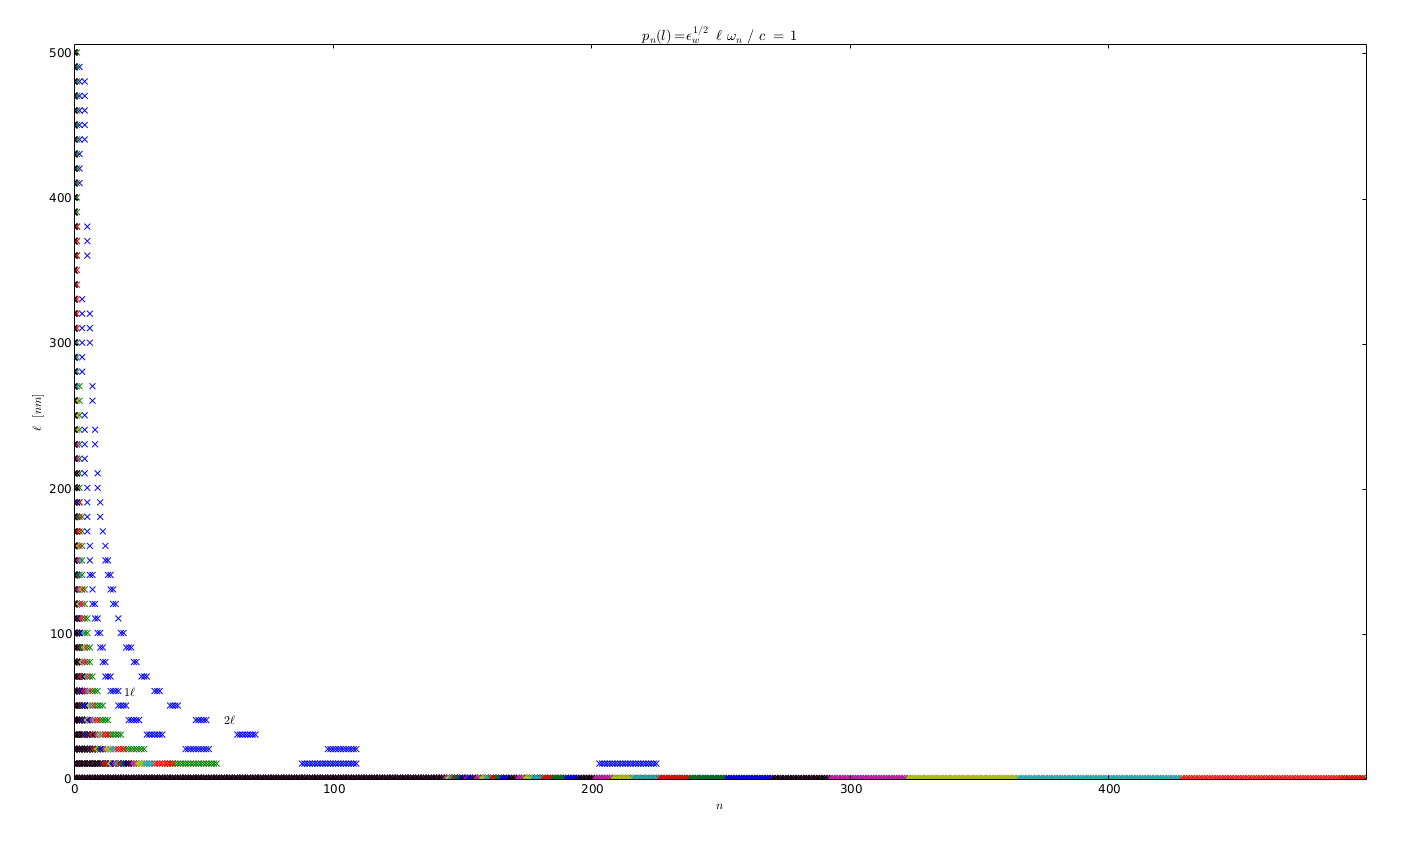
\includegraphics[width=1.2\textwidth,scale=0.8]{plots/p_vs_n_l.png}
%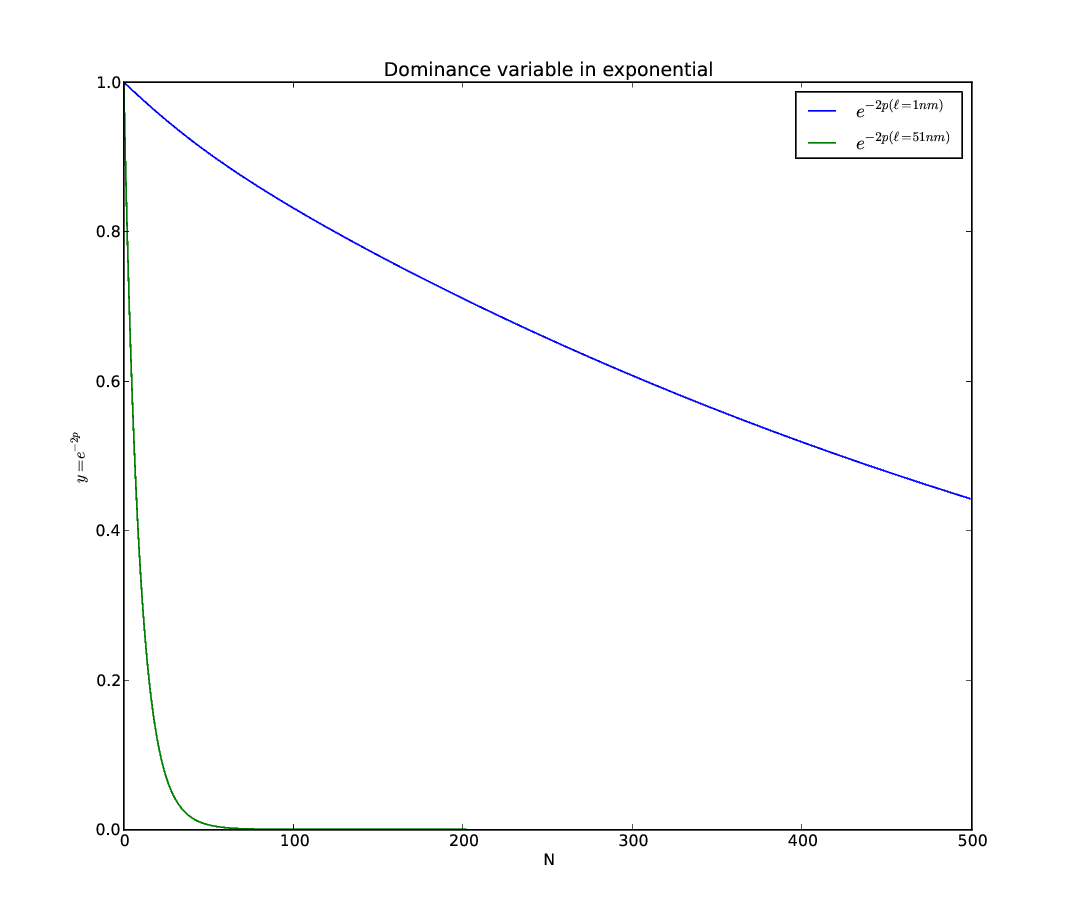
\includegraphics[width=1.2\textwidth]{plots/140415_93_n0_Dominance_variable_kink.png}
\hskip 43pt
\caption{Plot of values of n,$\ell$ for which $p_n(\ell)=1$.  Blue stars with
    the label "$1\ell$" are solutions to $p_n(\ell)=1$ for travel time from $cylinder_1$ to
    $cylinder_2$, but not back to $cylinder_1$. Blue stars with
    the label "$2\ell$" are solutions to $p_n(\ell)=1$ for travel time from $cylinder_1$ to
    $cylinder_2$ and back to $cylinder_1$. Stars of other colors represent
solutions to $p_n(\ell) < 1$.}
\label{eiz65}
\end{center}
\end{figure*} 

%\subsection{Plots of how each Matsubara term contributes to $\cal{A}_{n}^{(0)}(\ell)$}
%\subsection{Derivatives of Matsubara terms for $\cal{A}^{(0)}$ with respect
%to separation and n}
\begin{figure*}[t!]
\begin{center}
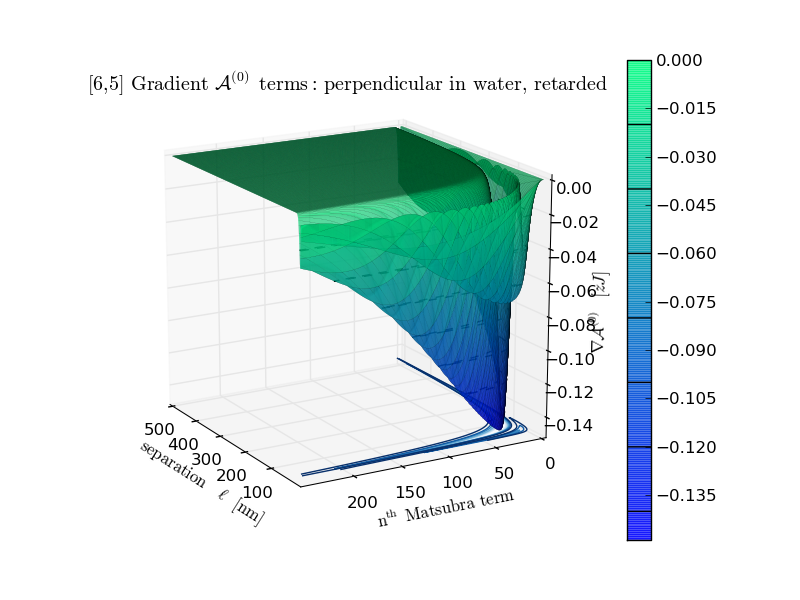
\includegraphics[width=1.4\textwidth]{plots/grad_A0_65.png}
\hskip 43pt
\caption{{\bf Derivative of ${\cal A}_{n}^{(0)}(\ell))$ for [6,5] with resepct to
$n$ and separation.}  Valleys in this 3D surface plot correspond to the
infection points in $\it{d}{\cal A}^{(0)}/\it{d}\ell$ of fig. 11 of previous
section and the solutions to  $p_n(\ell)=1$ in fig. 14 above.}
%derivative of
%$\cal{A}_{n}^{(0)}(\ell)$ (z-axis) with respect to separation and n (x and
%y axes. $Max[\lvert \nabla(\cal{A}^{(0)}) \rvert]$ occurs at
%$\ell=\ell_{knee}$}
\label{eiz65}
\end{center}
\end{figure*} 
\end{center}
%\begin{figure*}[t!]
%\begin{center}
%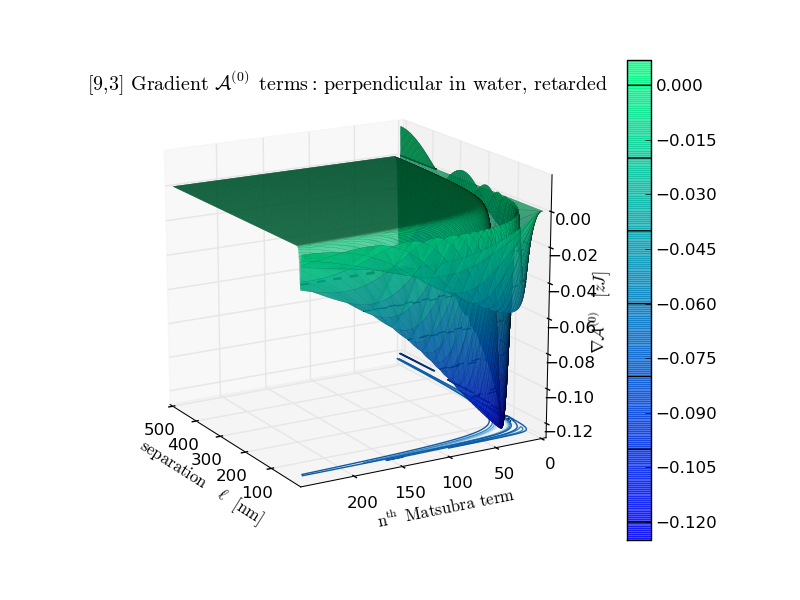
\includegraphics[width=1.4\textwidth]{plots/grad_A0_93.png}
%\hskip 43pt
%\caption{$\nabla(\cal{A}_{n}^{(0)}(\ell))$ for [9,3]: derivative of
%$\cal{A}_{n}^{(0)}(\ell)$ (z-axis) with respect to separation and n (x and
%y axes. $Max[\lvert \nabla(\cal{A}^{(0)}) \rvert]$ occurs at
%$\ell=\ell_{knee}$}
%\label{eiz65}
%\end{center}
%\end{figure*} 
%

%%%%%%%%%%%%%%%%%%%%%% SIBER COMPARE %%%%%%%%%%%%%%%%%%%%%%%%%%%%%%%%%%%%%%%%%%%%%%%%%
\section{Comparison to Siber plots: in progress (the plots shown here need a
correction to the n=0 terms)}

\subsection{[9,3] semi-conductor: retarded and non-retarded free energies}
\begin{figure*}[t!]
\begin{center}
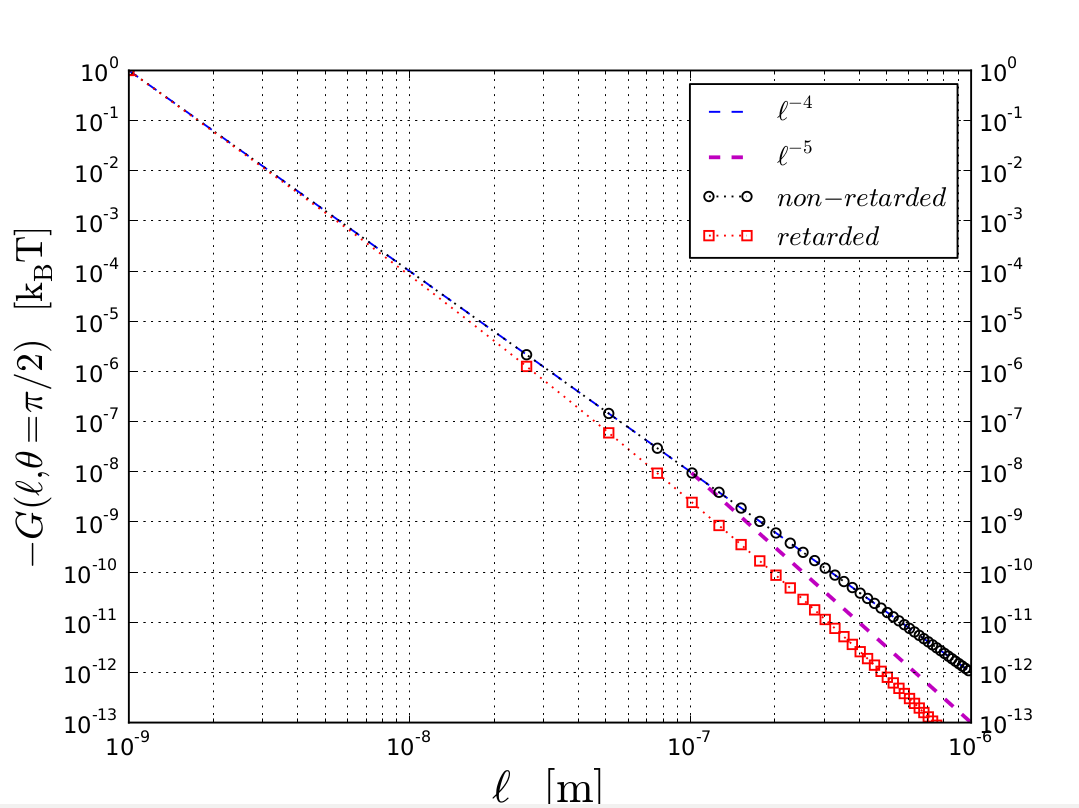
\includegraphics[width=1.5\textwidth]{plots/siber_comp_G_vs_l_sw_r_nr_65.png}
\hskip 43pt
\caption{$\cal{G}(\ell)$ for [6,5] in water}
\label{eiz65}
\end{center}
\end{figure*} 

\begin{figure*}[t!]
\begin{center}
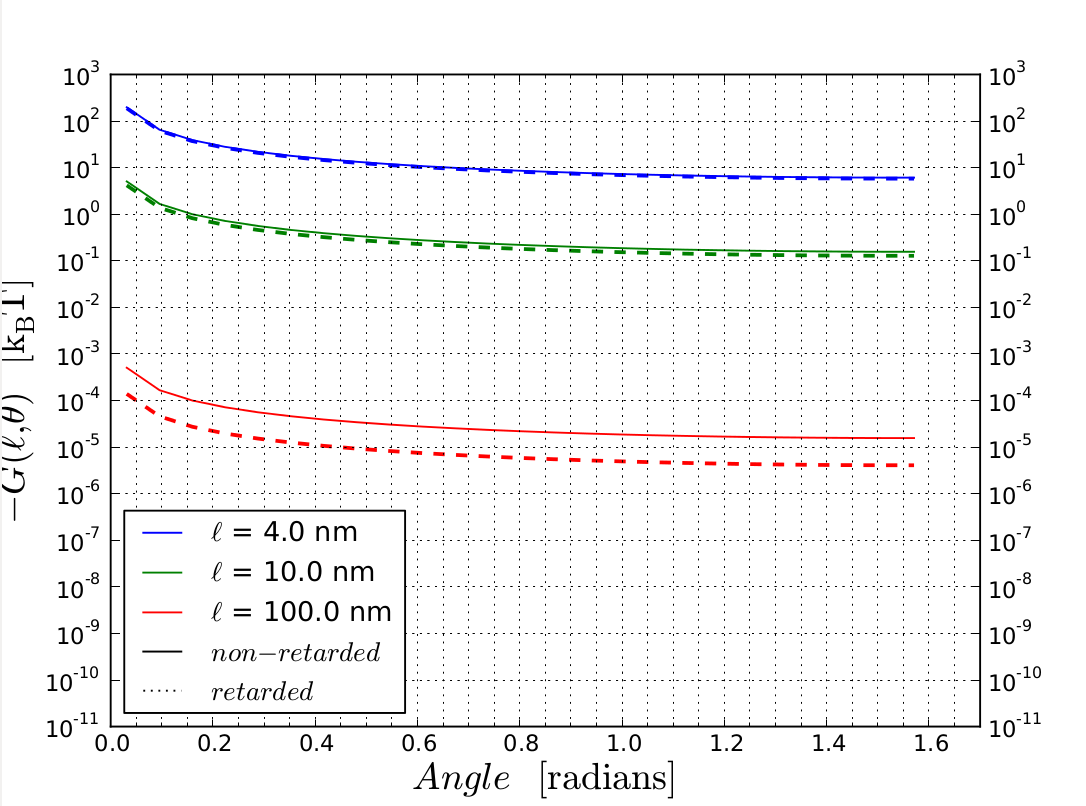
\includegraphics[width=1.5\textwidth]{plots/siber_comp_G_vs_theta_65.png}
\hskip 43pt
\caption{$\cal{G}(\theta)$ for [6,5] in water}
\label{eiz65}
\end{center}
\end{figure*} 

\end{center}

\end{document}







